\PassOptionsToPackage{unicode=true}{hyperref} % options for packages loaded elsewhere
\PassOptionsToPackage{hyphens}{url}
%
\documentclass[]{article}
\usepackage{lmodern}
\usepackage{amssymb,amsmath}
\usepackage{ifxetex,ifluatex}
\usepackage{fixltx2e} % provides \textsubscript
\ifnum 0\ifxetex 1\fi\ifluatex 1\fi=0 % if pdftex
  \usepackage[T1]{fontenc}
  \usepackage[utf8]{inputenc}
  \usepackage{textcomp} % provides euro and other symbols
\else % if luatex or xelatex
  \usepackage{unicode-math}
  \defaultfontfeatures{Ligatures=TeX,Scale=MatchLowercase}
\fi
% use upquote if available, for straight quotes in verbatim environments
\IfFileExists{upquote.sty}{\usepackage{upquote}}{}
% use microtype if available
\IfFileExists{microtype.sty}{%
\usepackage[]{microtype}
\UseMicrotypeSet[protrusion]{basicmath} % disable protrusion for tt fonts
}{}
\IfFileExists{parskip.sty}{%
\usepackage{parskip}
}{% else
\setlength{\parindent}{0pt}
\setlength{\parskip}{6pt plus 2pt minus 1pt}
}
\usepackage{hyperref}
\hypersetup{
            pdfborder={0 0 0},
            breaklinks=true}
\urlstyle{same}  % don't use monospace font for urls
\usepackage[paper=a4paper,lmargin=2cm, rmargin=2cm, tmargin=2cm, bmargin=2cm]{geometry}
\usepackage{longtable,booktabs}
% Fix footnotes in tables (requires footnote package)
\IfFileExists{footnote.sty}{\usepackage{footnote}\makesavenoteenv{longtable}}{}
\usepackage{graphicx,grffile}
\makeatletter
\def\maxwidth{\ifdim\Gin@nat@width>\linewidth\linewidth\else\Gin@nat@width\fi}
\def\maxheight{\ifdim\Gin@nat@height>\textheight\textheight\else\Gin@nat@height\fi}
\makeatother
% Scale images if necessary, so that they will not overflow the page
% margins by default, and it is still possible to overwrite the defaults
% using explicit options in \includegraphics[width, height, ...]{}
\setkeys{Gin}{width=\maxwidth,height=\maxheight,keepaspectratio}
\setlength{\emergencystretch}{3em}  % prevent overfull lines
\providecommand{\tightlist}{%
  \setlength{\itemsep}{0pt}\setlength{\parskip}{0pt}}
\setcounter{secnumdepth}{5}
% Redefines (sub)paragraphs to behave more like sections
\ifx\paragraph\undefined\else
\let\oldparagraph\paragraph
\renewcommand{\paragraph}[1]{\oldparagraph{#1}\mbox{}}
\fi
\ifx\subparagraph\undefined\else
\let\oldsubparagraph\subparagraph
\renewcommand{\subparagraph}[1]{\oldsubparagraph{#1}\mbox{}}
\fi

% set default figure placement to htbp
\makeatletter
\def\fps@figure{htbp}
\makeatother

\usepackage[portuguese]{babel}
\usepackage[utf8]{inputenc}
\usepackage[T1]{fontenc}
\usepackage{amsthm,amssymb,amsfonts,amsmath}
\usepackage{bm}
\usepackage{setspace}
\usepackage{multirow}
\usepackage{booktabs}
\usepackage{graphicx}
\usepackage{enumerate}
\usepackage{times}
\usepackage{xcolor}
\usepackage{csquotes}
\usepackage{natbib}
\usepackage{xcolor}

\addto\captionsportuguese{
      \renewcommand{\contentsname}%
        {Sumário}%
  }
  
\newlength{\drop}


\newcommand{\HRule}{\rule{\linewidth}{0.5mm}}

\usepackage[all]{background}

\backgroundsetup{
placement=center,
scale=1.5,
color=black,
opacity=0.075,
angle=0,
contents={
  
\includegraphics[width=0.65\linewidth]{logo-ufba}
  }
}

\DeclareMathOperator{\vari}{Var}
\DeclareMathOperator{\espe}{E}
\DeclareMathOperator*{\argmax}{arg\,max}
\DeclareMathOperator*{\argmin}{arg\,min}

\author{}
\date{\vspace{-2.5em}}

\begin{document}

\onehalfspacing

\begin{titlepage}
    \drop=0.1\textheight
    \centering
    \vspace*{\baselineskip}
    \rule{\textwidth}{1.6pt}\vspace*{-\baselineskip}\vspace*{2pt}
    \rule{\textwidth}{0.4pt}\\[\baselineskip]
    {\LARGE RELATÓRIO FINAL \\ 
    \vspace*{\baselineskip}
    INFÂNCIA EM TEMPOS DE PANDEMIA: EXPERIÊNCIAS DE CRIANÇAS 8 A 12 ANOS DURANTE O ISOLAMENTO SOCIAL EM DIFERENTES CONTEXTOS}\\[0.2\baselineskip]
    \rule{\textwidth}{0.4pt}\vspace*{-\baselineskip}\vspace{3.2pt}
    \rule{\textwidth}{1.6pt}\\[\baselineskip]
    \scshape
    Trabalho de consultoria realizado no contexto da ação de extensão da Universidade Federal da Bahia com título \textit{Consultoria Estatística}. \\
    \vspace*{2\baselineskip}
    Elaborado por \\[\baselineskip]
    {\Large Gilberto Pereira Sassi\par}
    \vfill
    {\scshape 2021} \\
    {\large Universidade Federal da Bahia}\\
    {\large Instituto de Matemática e Estatística}\\
    {\large Departamento de Estatística}\par
  \end{titlepage}

\newpage

\tableofcontents

\newpage

\hypertarget{introduuxe7uxe3o}{%
\section{Introdução}\label{introduuxe7uxe3o}}

Este relatório apresenta os resultados da análise estatística do conjunto de dados referente à seguinte consultoria:

\begin{itemize}
\tightlist
\item
  \textbf{Consulentes:} Profa. Dra. Juliana Prates Santana -- IPS/UFBA, e Profa. Dra. Adriana Ferriz -- IPS/UFBA;
\item
  \textbf{Título do projeto:} Infância em tempos de Pandemia: Experiências de crianças 8 a 12 anos
  durante o isolamento social em diferentes contextos.
\end{itemize}

O projeto tem o objetivo de analisar a percepção de crianças durante a pandemia de COVID-19 na região metropolitana de Salvador. As Consulentes solicitaram apoio para realizar comparações de médias de algumas escalas Likert. Mais especificamente, as consulentes desejam avaliar a influência das seguintes variáveis categóricas:

\begin{enumerate}
\def\labelenumi{\roman{enumi}.}
\tightlist
\item
  Idade
\item
  Tipo de escola
\item
  Gênero
\item
  Raça
\item
  Cidades
\end{enumerate}

nas seguintes variáveis que forem mensuradas como uma escala Likert:

\begin{enumerate}
\def\labelenumi{\roman{enumi}.}
\tightlist
\item
  Questão 12)
\item
  Questão 13)
\item
  Questão 14)
\item
  Questão 15)
\item
  Questão 16)
\item
  Questão 17)
\item
  Questão 18)
\item
  Questão 23)
\item
  Questão 29)
\end{enumerate}

\hypertarget{materias-e-muxe9todos}{%
\section{Materias e Métodos}\label{materias-e-muxe9todos}}

Começamos com uma análise descritiva de cada uma das variáveis de interesse, para depois passar para uma análise bidimensional. Na análise descritiva usamos medidas de posição e dispersão para variáveis mensuradas como uma escala Likert e tabela de distribuição de frequências para variáveis categóricas. Além disso, usamos o teste de associação qui-quadrado, o teste Kruskal-Wallis para comparar medianas e o teste de comparações múltiplas de Nemeyi. Neste projeto usamos a linguagem \texttt{R} (R Core Team \protect\hyperlink{ref-Rlang}{2021}). Para detalhes de estística descritiva, recomendamos a leitura de Bussab and Morettin (\protect\hyperlink{ref-bussab2002estatistica}{2002}). A seguir vamos apresentar detalhes metodológicos sobre o teste de associação qui-quadrado, o teste de Kruskal-Wallis para comparar medianas e o teste de comparações múltiplas de Nemeyi.

\hypertarget{teste-qui-quadrado}{%
\subsection{Teste qui-quadrado}\label{teste-qui-quadrado}}

Vamos começar definindo o que entendemos por associação entre duas variáveis.
Considere duas variáveis qualitativas \(X\) e \(Y\) com

\begin{itemize}
\tightlist
\item
  valores possíveis de \(X\): \(A_1, A_2, \dots, A_r\),
\item
  valores possíveis de \(Y\): \(B_1, B_2, \dots, B_s\).
\end{itemize}

Suponha que \(f_i \%\) da população de todos docentes tem valor de \(X\) igual \(A_i\).
Então,

\begin{enumerate}
\def\labelenumi{\arabic{enumi}.}
\tightlist
\item
  dizemos que \(X\) e \(Y\) estão associados se, ao descobrirmos ou conhecermos que o valor de
  \(Y\) é \(B_j\), \textbf{alteramos} o valor de \(f_i \%\);
\item
  dizemos que \(X\) e \(Y\) \textbf{não} estão associados se, ao descobrirmos ou conhecermos que o valor de
  \(Y\) é \(B_j\), \textbf{não alteramos} o valor de \(f_i \%\);
\end{enumerate}

Para verificar se duas variáveis qualitativas estão associadas usando uma amostra,
começamos construindo a tabela de contingência que mostra a frequência da variáveis
\(X\) ao longo da variávei \(Y\), conforme ilustrado na Tabela \ref{tab:contingencia}.

\begin{table}[htbp]
  \centering
  \caption{Tabela de contingência para as variáveis $X$ e $Y$.}
  \label{tab:contingencia}
  \begin{tabular}{c|c|ccccc|c}
    &  & \multicolumn{5}{|c|}{Valores possíveis de $X$} & \\ \cline{3-7}
    &  & $B_1$ & $B_2$ & $B_3$ & $\cdots$ & $B_s$ & Total\\ \hline
  \multirow{5}{*}{Valores possíveis de $Y$}  & $A_1$ & $n_{11}$ & $n_{12}$ & $n_{13}$ & $\cdots$ & $n_{1s}$ & $n_{1\cdot}$ \\
    & $A_2$ & $n_{21}$ & $n_{22}$ & $n_{23}$ & $\cdots$ & $n_{2s}$ & $n_{2\cdot}$ \\
    & $A_3$ & $n_{31}$ & $n_{32}$ & $n_{33}$ & $\cdots$ & $n_{3s}$ & $n_{3\cdot}$ \\
    & $\vdots$ & $\vdots$ & $\vdots$ & $\vdots$ & $\ddots$ & $\vdots$ & $\vdots$\\
    & $A_r$ & $n_{r1}$ & $n_{r2}$ & $n_{r3}$ & $\cdots$ & $n_{rs}$ & $n_{r\cdot}$  \\ \hline
    & Total & $n_{\cdot 1}$ & $n_{\cdot 2}$ & $n_{\cdot 3}$ & $\cdots$ & $n_{\cdot s}$ & $n_{\cdot \cdot}$ 
  \end{tabular}
\end{table}

em que \(n_{ij}\) é o número de docentes que tem valor de \(X\) igual a \(A_i, i=1, \dots, r\) e tem valor de \(Y\) igual a \(B_j, j=1, \dots, s\); \(n_{i\cdot}\)
é o número de docentes que tem valor de \(X\) igual a \(A_i, i=1, \dots, r\);
\(n_{\cdot j}, j=1, \dots, s\) é o número de docentes que tem valor de \(Y\) igual a
\(B_j, j=1, \dots, s\); e \(n_{\cdot \cdot}\) é o tamanho da amostra. Para verificar se duas variáveis estão associadas, podemos
calcular a frequência relativa por colunas (ou por linhas), conforme ilustrado na
Tabela \ref{tab:FRContingencia}.

\begin{table}[htbp]
  \centering
  \caption{Frequência relativa por coluna da tabela de contingência para as variáveis $X$ e $Y$.}
  \label{tab:FRContingencia}
  \begin{tabular}{c|c|ccccc|c}
    &  & \multicolumn{5}{|c|}{Valores possíveis de $X$} & \\ \cline{3-7}
    &  & $B_1$ & $B_2$ & $B_3$ & $\cdots$ & $B_s$ & Total\\ \hline
  \multirow{5}{*}{Valores possíveis de $Y$}  & $A_1$ & $\frac{n_{11}}{n{\cdot 1}}$ & $\frac{n_{12}}{n_{\cdot 2}}$ & $\frac{n_{13}}{n_{\cdot 3}}$ & $\cdots$ & $\frac{n_{1s}}{n_{\cdot s}}$ & $\frac{n_{1\cdot}}{n_{\cdot \cdot}}$ \\
    & $A_2$ & $\frac{n_{21}}{n_{\cdot 1}}$ & $\frac{n_{22}}{n_{\cdot 2}}$ & $\frac{n_{23}}{n_{\cdot 3}}$ & $\cdots$ & $\frac{n_{2s}}{n_{\cdot s}}$ & $\frac{n_{2\cdot}}{n_{\cdot \cdot}}$ \\
    & $A_3$ & $\frac{n_{31}}{n_{\cdot 1}}$ & $\frac{n_{32}}{n_{\cdot 2}}$ & $\frac{n_{33}}{n_{\cdot 3}}$ & $\cdots$ & $\frac{n_{3s}}{n_{\cdot s}}$ & $\frac{n_{3\cdot}}{n_{\cdot \cdot}}$ \\
    & $\vdots$ & $\vdots$ & $\vdots$ & $\vdots$ & $\ddots$ & $\vdots$ & $\vdots$\\
    & $A_r$ & $\frac{n_{r1}}{n_{\cdot 1}}$ & $\frac{n_{r2}}{n_{\cdot 2}}$ & $\frac{n_{r3}}{n_{\cdot 3}}$ & $\cdots$ & $\frac{n_{rs}}{n_{\cdot s}}$ & $\frac{n_{r\cdot}}{n_{\cdot \cdot}}$  \\ \hline
    & Total & $\frac{n_{\cdot 1}}{n_{\cdot 1}} = 1$ & $\frac{n_{\cdot 2}}{n_{\cdot 2}}=1$ & $\frac{n_{\cdot 3}}{n_{\cdot 3}} = 1$ & $\cdots$ & $\frac{n_{\cdot s}}{n_{\cdot s}} = 1$ & $\frac{n_{\cdot \cdot}}{n_{\cdot \cdot}}=1$ 
  \end{tabular}
\end{table}

Se \(X\) e \(Y\) não estão associadas, então, para cada linha \(i, i=1, \dots, r\) da Tabela \ref{tab:FRContingencia},
temos que
\begin{equation}
\frac{n_{ij}}{n_{\cdot j}} = \frac{n_{i\cdot }}{n_{\cdot \cdot}}, i=1, \dots, r,
\label{eq:equality}
\end{equation}
e podemos analisar essas igualdades usando um gráfico de barras e usando o teste
qui-quadrado, como explicaremos a seguir.

Para ilustrar a associação e a não associção entre duas variáveis qualitativas,
vamos considerar dois exemplos didáticos que podem ser encontrados no livro de
Barbetta (\protect\hyperlink{ref-barbetta2008estatistica}{2008}).

\hypertarget{exemplo-de-associauxe7uxe3o-entre-duas-variuxe1veis-qualitativas}{%
\subsubsection{Exemplo de associação entre duas variáveis qualitativas}\label{exemplo-de-associauxe7uxe3o-entre-duas-variuxe1veis-qualitativas}}

Para ilustração vamos estudar um exempo de não associação hipotético do livro Barbetta (\protect\hyperlink{ref-barbetta2008estatistica}{2008}). Imagine que um pesquisador está interessado em estudar a associação entre \texttt{câncer} e o \texttt{tabagismo} em uma amostra com 300 indivíduos e obteve a tabela de contingência mostrada na Tabela \ref{tab:associacao}. A variável \texttt{câncer} tem duas categorias: \texttt{sim} (a pessoa teve ou tem câncer); \texttt{não} (a pessoa não teve nem tem câncer). A variável \texttt{tabagismo} tem duas categorias: \texttt{fumante} (a pessoa tem o hábito de fumar); \texttt{não-fumante} (a pessoa não tem hábito de fumar).

\begin{table}[htbp]
\centering
\caption{Tabela de distribuição de frequência entre Câncer e Tabagismo.}
\label{tab:associacao}
\begin{tabular}{l|cc|l}
    & \multicolumn{2}{|c|}{Câncer} & \\ \cline{2-3}
    Tabagismo & Não & Sim & Total\\ \hline
    Não-Fumante & 200 & 0 & 200 \\
    Fumante & 0 & 100 & 100\\ \hline
    Total & 200 & 100 & 300
\end{tabular}
\end{table}

Calculando a frequência relativa por linha na Tabela \ref{tab:associacao}, obtemos as frequências relativas da Tabela \ref{tab:associacaoRel}.

\begin{table}[htbp]
\centering
\caption{Tabela de distribuição de frequência relativa ao total das linhas.}
\label{tab:associacaoRel}
\begin{tabular}{l|ll|l}
& \multicolumn{2}{|c|}{Câncer (Y)} & \\ \cline{2-3}
Tabagismo (X) & Não & Sim & Total\\ \hline
Não-Fumante & $\frac{200}{200}\cdot 100 = 100\%$ & {\color{brown} $\frac{0}{200}\cdot 100 = 0\%$} & $\frac{200}{200}\cdot 100= 100\%$ \\
Fumante & $\frac{0}{100}\cdot 100 = 0\%$  & {\color{blue} $\frac{100}{100}\cdot 100= 100\%$} &  $\frac{100}{100}\cdot 100=100\%$ \\ \hline
Total & $\frac{200}{300}\cdot 100= 66,67\%$ & {\color{red} $\frac{100}{300}\cdot 100 = 33,33\%$}  & $\frac{300}{300}\cdot 100= 100\%$ 
\end{tabular}
\end{table}

Na Tabela \ref{tab:associacaoRel}, notamos que os valores destacados em vermelho, azul e marrom são diferentes. Se não sabemos o valor da variável \texttt{tabagismo} de um indivíduo, dizemos que ele tem aproximadamente \(33\%\) de probabilidade de ter câncer (conforme destacado em vermelhado). Contudo, ao descobrir / revelar / conhecer o valor da variável \texttt{tabagismo}, essa probabilidade muda. Mais precisamente, se descobrirmos que a pessoa fuma (\texttt{tabagismo} = \texttt{fumante}) então a probabilidade da pessoa ter cancer é aproximadamente \(100\%\), e se descobrirmos que a pessoa não fuma (\texttt{tabagismo} = \texttt{não-fumante}) então a probabildiade da pessoa ter câncer é aproximadamente \(0\%\). Ou seja, conhecer o valor \texttt{tabagismo} para uma pessoa muda, ou altera, as probabilidades dos valores de \texttt{câncer}, e então dizemos as duas variáveis qualitativas estão associadas. Geralmente, é conveniente representar a Tabela \ref{tab:associacaoRel} usando gráfico de barras conforme ilustrado na Figura \ref{fig:associacao}. Note que na Figura \ref{fig:associacao}, as duas barras são diferentes. De uma forma geral, se as barras iguais indicam uma não associação entre as variáveis qualitativas e barras diferentes indicam uma associação entre as variáveis qualitativas.

\begin{figure}[htbp]

{\centering 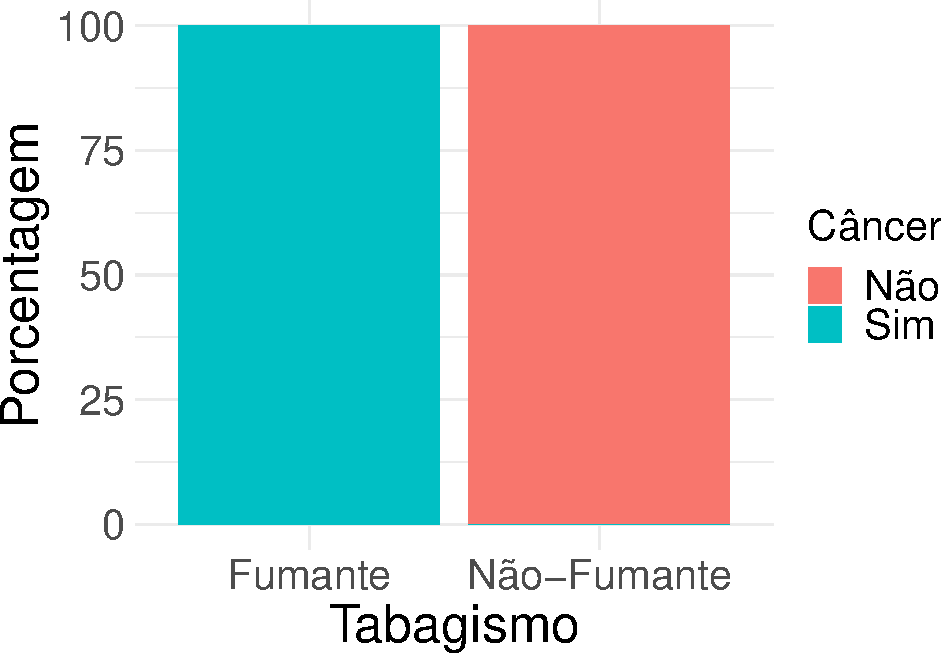
\includegraphics[width=0.5\linewidth]{relatorio_files/figure-latex/associacao-1} 

}

\caption{Associação entre Tabagismo e Câncer.}\label{fig:associacao}
\end{figure}

\hypertarget{exemplo-de-nuxe3o-associauxe7uxe3o-entre-duas-variuxe1veis-qualitativas}{%
\subsubsection{Exemplo de não associação entre duas variáveis qualitativas}\label{exemplo-de-nuxe3o-associauxe7uxe3o-entre-duas-variuxe1veis-qualitativas}}

Para ilustração vamos estudar um exempo de não associação hipotético do livro Barbetta (\protect\hyperlink{ref-barbetta2008estatistica}{2008}). Imagine que um pesquisador está interessado em estudar a associação entre as variáveis qualitativas \texttt{gênero} e \texttt{tabagismo} em uma amostra de \(300\) pessoas e obteve a tabela de contingência da Tabela \ref{tab:naoAssociacao}. A variável \texttt{gênero} tem duas categorias: \texttt{masculino} (a pessoa se identifica com o gênero masculino) e \texttt{feminino} (a pessoa se identifica com o gênero feminino). A variável \texttt{tabagismo} tem duas categorias: \texttt{fumante} (a pessoa tem o hábito de fumar) e \texttt{não-fumante} (a pessoa não tem o hábito de fumar).

\begin{table}[htbp]
\centering
\caption{Tabela de contingência para as Gênero e Tabagismo.}
\label{tab:naoAssociacao}
\begin{tabular}{l|cc|l}
& \multicolumn{2}{|c|}{Gênero} & \\ \cline{2-3}
Tabagismo & Masculino & Feminino & Total\\ \hline
Não-Fumante & 80 & 40 & 120\\
Fumante & 120 & 60 & 180\\ \hline
Total & 200 & 100 & 300\\
\end{tabular}
\end{table}

Calculando a frequência relativa por linha na Tabela \ref{tab:naoAssociacao}, obtemos as frequências relativas da Tabela \ref{tab:naoAssociacaoRel}.

\begin{table}[htbp]
\centering
\caption{Tabela de distribuição de frequência relativa ao total das colunas.}
\label{tab:naoAssociacaoRel}
\begin{tabular}{l|ll|l}
& \multicolumn{2}{|c|}{Gênero} & \\ \cline{2-3}
Tabagismo & Homem & Mulher & Total\\ \hline
Não-Fumante & {\color{brown} $\frac{80}{200}\cdot 100 = 40\%$} &  {\color{blue}$\frac{40}{100}\cdot 100 = 40\%$} & {\color{red}$\frac{120}{300}\cdot 100= 40\%$} \\
Fumante & $\frac{120}{200}\cdot 100 = 60\%$  &  $\frac{60}{100}\cdot 100= 60\%$ &  $\frac{180}{300}\cdot 100=60\%$ \\ \hline
Total & $\frac{200}{200}\cdot 100= 100\%$ &  $\frac{100}{100}\cdot 100 = 100\%$  & $\frac{300}{300}\cdot 100= 100\%$ \\ 
\end{tabular}
\end{table}

Na Tabela \ref{tab:naoAssociacaoRel}, notamos que os valores destacados em vermelho, azul e marrom são iguais. Se não sabemos o valor da variável \texttt{gênero} de um indivíduo, dizemos que uma pessoa tem aproximadamente \(40\%\) de probabilidade de ser fumante (conforme destacado em vermelhado). Contudo, ao descobrir / revelar / conhecer o valor da variável \texttt{gênero}, essa probabilidade permanece idêntica. Mais precisamente, se descobrirmos que a pessoa se identifica com o gênero feminino (\texttt{gênero} = \texttt{feminino}) então a probabilidade da pessoa fumar é aproximadamente \(40\%\) (cor azul), e se descobrirmos que a pessoa se identifica com o gênero masculino (\texttt{gênero} = \texttt{masculino}) então a probabildiade da pessoa fumar também é aproximadamente \(40\%\) (cor marrom). Ou seja, conhecer o valor \texttt{gênero} para uma pessoa não muda nem se altera as probabilidades dos valores de \texttt{tabagismo}, e então dizemos as duas variáveis qualitativas não estão associadas. Isto é, conhecer o valor da variável \texttt{gênero} não nos ajuda a descobrir ou determinar o valor (ou a probabilidade dos valores) da variável \texttt{tabagismo}. Geralmente, é conveniente representar a Tabela \ref{tab:naoAssociacaoRel} usando gráfico de barras conforme ilustrado na Figura \ref{fig:naoAssociacao}. Note que na Figura \ref{fig:naoAssociacao}, as duas barras são idênticas. De uma forma geral, se as barras iguais indicam uma não associação entre as variáveis qualitativas e barras diferentes indicam uma associação entre as variáveis qualitativas.

\begin{figure}[htbp]

{\centering 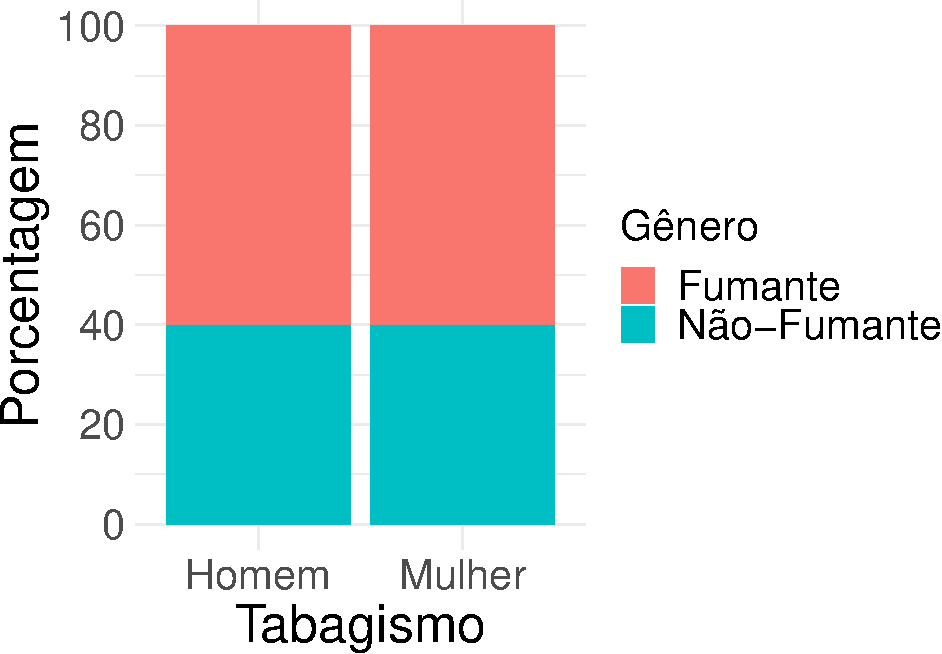
\includegraphics[width=0.5\linewidth]{relatorio_files/figure-latex/naoAssociacao-1} 

}

\caption{Não associação entre Gênero e Tabagismo.}\label{fig:naoAssociacao}
\end{figure}

\hypertarget{teste-qui-quadrado-1}{%
\subsubsection{Teste qui-quadrado}\label{teste-qui-quadrado-1}}

O teste qui-quadrado é geralmente usado para checar a associação entre duas variáveis
qualitativas. Considere as variáveis \(X\) e \(Y\) duas variáveis qualitativas da
Tabela \ref{tab:contingencia}, então, como já comentamos, se \(X\) e \(Y\) não são associadas temos que
\begin{equation}
\label{eq:quiQuadrado}
n_{ij} = \frac{n_{i \cdot } n_{\cdot j}}{n_{\cdot \cdot}} = \frac{\mbox{total da linha }i \cdot \mbox{total da colunha }j}{\mbox{tamanho da amostra}},
\end{equation}
em que \(n_{i \cdot}\) é o total da linha que corresponde ao valor \(A_i\) na Tabela \ref{tab:contingencia}, \(n_{\cdot j}\) é o total da colunha que corresponde ao valor \(B_j\) na Tabela \ref{tab:contingencia}, e \(n_{\cdot \cdot}\) é o tamanho da amostra.

Quando coletamos uma amostra não sabemos se duas variáveis estão associadas. Então, calculamos a expressão do lado direito da equação \eqref{eq:quiQuadrado}
\[
e_{ij} = \frac{\mbox{total da linha }i \cdot \mbox{total da colunha }j}{\mbox{tamanho da amostra}}
\]
e comparamos com o valor \(n_{ij}\) que obtemos da amostra. Chamamos \(e_{ij}\) de valor frequência esperada e \(n_{ij}\) de valor de frequência observada. Se as frequências esperadas e as frequência observadas forem iguais (ou estiverem próximas), podemos concluir que \(X\) e \(Y\) não estão associadas. Ou seja, se as distâncias padronizadas \(\frac{(e_{ij} - n_{ij})^2}{e_{ij}}\) entre \(e_{ij}\) e \(n_{ij}\) forem pequenas, então \(X\) e \(Y\) \textbf{não} estão associadas. Estas distâncias padronizadas são não-negativas, então \(X\) e \(Y\) \textbf{não} estão associadas se, e somente se, a soma de todas estas distâncias \(\frac{(e_{ij} - n_{ij})^2}{e_{ij}}\) são pequenas. Consequentemente, se
\[
\chi_0^2 = \sum_{i=1}^{r} \sum_{j=1}^{s} \frac{(e_{ij} - n_{ij})^2}{e_{ij}},
\]
for pequeno, então \(X\) e \(Y\) não estão associadas.

Para saber se \(\chi_0^2\) é pequeno ou grande, comparamos \(\chi_0^2\) o valor de quantil da distribuição qui-quadrado com \((r-1)(s-1)\) graus de liberdade (vide Montgomery and Runger \protect\hyperlink{ref-montgomery2010applied}{2010} para detalhes). Mais precisamente, queremos decidir entre as duas hipóteses científicas
\begin{align*}
H_0 &= \mbox{as duas variáveis qualitativas não estão associadas},\\
H_1 &= \mbox{as duas variáveis qualitativas estão associadas},
\end{align*}
e para isso fixamos o nível de significância \(\alpha\), calculamos o valor-p \(p\) e rejeitamos \(H_0\) se \(p < \alpha\) (vide Spiegel et al. \protect\hyperlink{ref-spiegel2001probability}{2001} para detalhes sobre valor-p). Neste relatório, vamos usar o nível de significânica \(\alpha=0,05\) .

\hypertarget{teste-kruskal-wallis}{%
\subsection{Teste Kruskal-Wallis}\label{teste-kruskal-wallis}}

Usamos o Teste Kruskal-Wallis para comparar populações através da mediana e adequado para populações onde não é adequado assumir a distribuição normal, como é caso escalas Likert. Neste teste, supomos que temos \(j,\quad j=1, \dots, k\) populações e para cada população \(j\) temos coletamos uma amostra de tamanho \(n_j\), ou seja, a amostra completa tem \(N = n_1 + \dots + n_k\) crianças. Seja \(X_{ij}\) é a resposta da criança \(i\) da população \(j\), então
\[
X_{ij} = \theta + \tau_j + \epsilon_{ij}, \qquad  j=1, \dots, k,\qquad i=1, \dots, n_j,
\]
onde \(\theta\) é a mediana da amostra completa, \(\tau_j\) é o efeito do \(j\)-ésimo tratamento da população e \(\epsilon_{ij}\) são erros aleatórios com mediana igual a zero, e queremos decidir entre duas hipóteses
\[
\begin{split}
&H_0: \tau_1 = \tau_2 = \dots = \tau_j,\\
&H_1: \tau_1, \tau_2, \dots,  \tau_j \mbox{ não são todos iguais}.
\end{split}
\]
e para isso fixamos o nível de significância \(\alpha\), calculamos o valor-p \(p\) e rejeitamos \(H_0\) se \(p < \alpha\) (vide Spiegel et al. \protect\hyperlink{ref-spiegel2001probability}{2001} para detalhes sobre valor-p). Neste relatório, vamos usar o nível de significânica \(\alpha=0,05\).

Para detalhes sobre o teste Kruskal-Wallis, recomendo a leitura de Hollander, Wolfe, and Chicken (\protect\hyperlink{ref-hollander2013nonparametric}{2013}).

\hypertarget{teste-de-comparauxe7uxe3o-muxfaltipla-de-nemeyi}{%
\subsection{Teste de comparação múltipla de Nemeyi}\label{teste-de-comparauxe7uxe3o-muxfaltipla-de-nemeyi}}

O teste de Nemeyi (Nemenyi \protect\hyperlink{ref-nemenyi1963distribution}{1963}) é teste \emph{posthoc} de comparação múltipla que pode ser usada para identificar quais grupos tem medianas diferentes populações se o teste de Kruskal-Wallis indica que as populações tem medianas diferentes. O teste consiste em realizar comparações em pares para identificar quais populações tem medianas diferentes.

O número de comparações de medianas realizadas é \(\frac{k(k-1)}{2}\), e o teste foi construído em soma de postos e na aplicação do método \emph{family-wise-error} para controlar a inflação do erro tipo I se várias comparações forem feitas. E para cada par de populações queremos decidir entre as hipóteses:
\[
\begin{split}
&H_0: m_l = m_j\\
&H_1: m_l \neq m_j
\end{split}
\]
onde \(m_l\) é a mediana da população \(l\) e \(m_j\) é a mediana da população \(j\). Para decidirmos entre estas hipóteses, fixamos o nível de significância \(\alpha\), calculamos o valor-p \(p\) e rejeitamos \(H_0\) se \(p < \alpha\) (vide Spiegel et al. \protect\hyperlink{ref-spiegel2001probability}{2001} para detalhes sobre valor-p). Neste relatório, vamos usar o nível de significânica \(\alpha=0,05\).

Para detalhes sobre o teste de comparação múltipla de Nemeyi, recomendo a leitura da vinheta do pacote da liguagem Pohlert (\protect\hyperlink{ref-PMCMR}{2014}).

\hypertarget{arquivos-suplementares}{%
\subsection{Arquivos suplementares}\label{arquivos-suplementares}}

Para facilitar a redação de relatórios e artigos pelas consulentes, coloco em anexo os seguintes arquivos:

\begin{itemize}
\tightlist
\item
  \texttt{output.zip}: este arquivo contém o sequintes diretórios

  \begin{itemize}
  \tightlist
  \item
    \texttt{kruskal\_wallis\_test}: diretório com arquivos \texttt{.csv} e \texttt{.xlsx} com os testes Kruskal-Wallis
  \item
    \texttt{medidas\_resumos\_bidimensional}: diretório com arquivos \texttt{.csv} e \texttt{.xlsx} com medidas de resumo calculas de cada grupo de uma variável categórica
  \item
    \texttt{medidas\_resumos\_unidimensional}: diretório com arquivos \texttt{.csv} e \texttt{.xlsx} com medidas de resumo para cada uma das variáveis neste relatório
  \item
    \texttt{nemenyi\_tests}: diretório com arquivos \texttt{.csv} e \texttt{.xlsx} com os valores-p do teste de comparação múltipla de Nemeyi
  \item
    \texttt{tabela\_contingencia}: diretório com arquivos \texttt{.csv} e \texttt{.xlsx} com as tabelas de contingências
  \item
    \texttt{tabela\_distribuicao}: diretório com arquivos \texttt{.csv} e \texttt{.xlsx} com as tabelas de distribuições de frequências para as variáveis categóricas
  \item
    \texttt{teste\_qui\_quadrado}: diretório com arquivos \texttt{.csv} e \texttt{.xlsx} com os testes qui-quadrado
  \end{itemize}
\item
  \texttt{figuras.zip}: este arquivo contém os seguintes diretórios:

  \begin{itemize}
  \tightlist
  \item
    \texttt{boxplot\_bidimensional}: diretório com figuras nos formatos \texttt{.png} e \texttt{.pdf} com o diagrama de caixa (boxplot) de cada grupo da variável categórica
  \item
    \texttt{grafico\_barra\_bidimensional}: diretório com figuras nos formatos \texttt{.png} e \texttt{.pdf} com gráfico de barras para duas variáveis categóricas
  \item
    \texttt{grafico\_barra\_unidimensional}: diretório com figuras nos formatos \texttt{.png} e \texttt{.pdf} com gráfico de barras para cada variável categórica
  \end{itemize}
\end{itemize}

\cleardoublepage

\hypertarget{resultados}{%
\section{Resultados}\label{resultados}}

Dividimos esta seção em duas partes. Começamos com a análise descritiva para as seguintes variávies categóricas:

\begin{enumerate}
\def\labelenumi{\roman{enumi}.}
\tightlist
\item
  Idade
\item
  Tipo de escola
\item
  Gênero
\item
  Raça
\item
  Cidades
\end{enumerate}

Nesta parte, apresentamos as tabelas de distribuição de frequências e o gráfico de barras sem comentários adicionais. Em seguida, comparamos as escalas de Likert por cada grupo especificado pelas variáveis categóricas elencadas acima. Nesta última parte, também seremos lacônicos, pois este relator acredita que as consulentes são qualificadas para dar uma interpretação adequada aos resultados dos métodos estatísticos.

\cleardoublepage

\hypertarget{q12}{%
\subsection{Q12}\label{q12}}

A variável Q12 corresponde a questão 13 com enunciado \textbf{No início da pandemia de coronavírus, o quanto você se preocupou com as questões abaixo:} no quesito:

\begin{itemize}
\tightlist
\item
  \emph{Que demorasse muito para eu voltar à escola?}
\end{itemize}

\hypertarget{anuxe1lise-descritiva-para-q12}{%
\subsubsection{Análise descritiva para Q12}\label{anuxe1lise-descritiva-para-q12}}

\hypertarget{gruxe1fico-de-barras-q12}{%
\paragraph{Gráfico de barras: Q12}\label{gruxe1fico-de-barras-q12}}

\begin{center}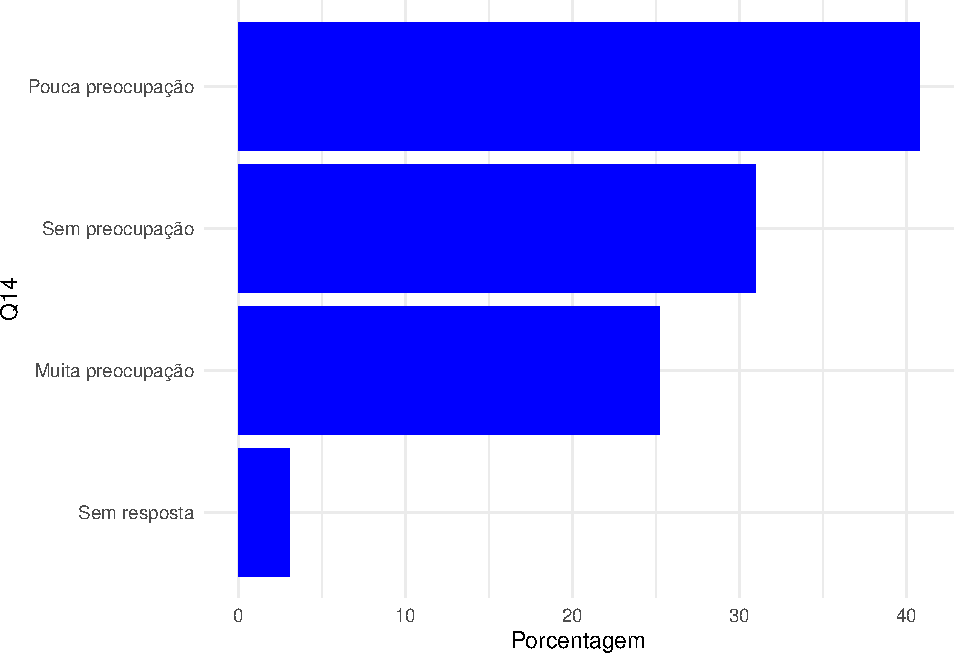
\includegraphics[width=0.75\linewidth]{relatorio_files/figure-latex/unnamed-chunk-14-1} \end{center}

\hypertarget{tabela-de-distribuiuxe7uxe3o-q12}{%
\paragraph{Tabela de distribuição: Q12}\label{tabela-de-distribuiuxe7uxe3o-q12}}

\begin{longtable}[]{@{}cccc@{}}
\caption{\label{tab:unnamed-chunk-15}Você está preocupado que demorasse muito para eu voltar à escola?}\tabularnewline
\toprule
Q12 & Frequência & Frequência relativa & Porcentagem\tabularnewline
\midrule
\endfirsthead
\toprule
Q12 & Frequência & Frequência relativa & Porcentagem\tabularnewline
\midrule
\endhead
Pouca preocupação & 430 & 0,41 & 40,95\tabularnewline
Muita preocupação & 389 & 0,37 & 37,05\tabularnewline
Sem preocupação & 204 & 0,19 & 19,43\tabularnewline
Sem resposta & 27 & 0,03 & 2,57\tabularnewline
\bottomrule
\end{longtable}

\hypertarget{medidas-de-resumo-q12}{%
\paragraph{Medidas de resumo: Q12}\label{medidas-de-resumo-q12}}

\begin{longtable}[]{@{}ccccc@{}}
\caption{\label{tab:unnamed-chunk-16}Resumos para variável Q12.}\tabularnewline
\toprule
Média & Desvio Padrão & Mediana & 1Qua & 3Qua\tabularnewline
\midrule
\endfirsthead
\toprule
Média & Desvio Padrão & Mediana & 1Qua & 3Qua\tabularnewline
\midrule
\endhead
1,23 & 0,79 & 1 & 1 & 2\tabularnewline
\bottomrule
\end{longtable}

\cleardoublepage

\hypertarget{anuxe1lise-bidimensional-para-q12}{%
\subsubsection{Análise bidimensional para Q12}\label{anuxe1lise-bidimensional-para-q12}}

\hypertarget{tabela-de-continguxeancia-cidade-e-q12}{%
\paragraph{Tabela de contingência: Cidade e Q12}\label{tabela-de-continguxeancia-cidade-e-q12}}

\begin{longtable}[]{@{}ccccc@{}}
\caption{\label{tab:unnamed-chunk-17}Tabela de contingência: Cidade e Q12.}\tabularnewline
\toprule
Cidade & Muita preocupação & Pouca preocupação & Sem preocupação & Sem resposta\tabularnewline
\midrule
\endfirsthead
\toprule
Cidade & Muita preocupação & Pouca preocupação & Sem preocupação & Sem resposta\tabularnewline
\midrule
\endhead
Camaçari & 87 & 82 & 22 & 6\tabularnewline
Candeias & 16 & 13 & 8 & 1\tabularnewline
Lauro de Freitas & 16 & 26 & 19 &\tabularnewline
Outros & 33 & 35 & 15 &\tabularnewline
Pojuca & 25 & 33 & 6 &\tabularnewline
Salvador & 204 & 225 & 125 & 19\tabularnewline
Simões Filho & 8 & 16 & 9 & 1\tabularnewline
\bottomrule
\end{longtable}

\hypertarget{gruxe1fico-de-barras-cidade-e-q12}{%
\paragraph{Gráfico de barras: Cidade e Q12}\label{gruxe1fico-de-barras-cidade-e-q12}}

Aparentemente as duas variáveis \emph{Cidade} e \emph{Q12} estão associadas.

\begin{center}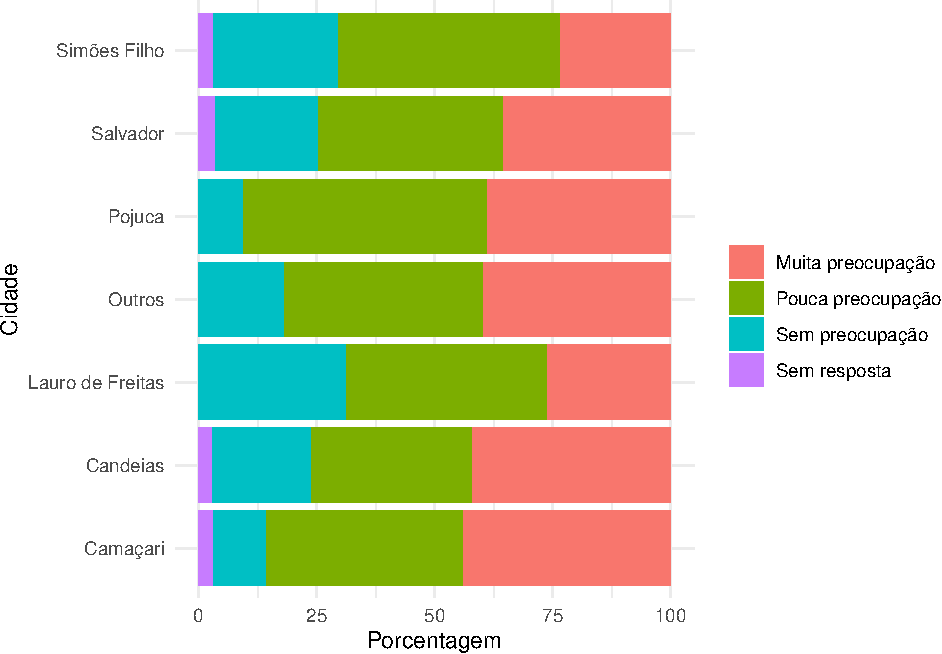
\includegraphics[width=0.75\linewidth]{relatorio_files/figure-latex/unnamed-chunk-18-1} \end{center}

\hypertarget{teste-qui-quadrado-2}{%
\paragraph{Teste qui-quadrado}\label{teste-qui-quadrado-2}}

Como o valor-p é menor que \(\alpha=0,05\), rejeitamos \(H_0\) e temos evidência evidência estatística que as duas variáveis estão associadas.

\begin{longtable}[]{@{}ccc@{}}
\caption{\label{tab:unnamed-chunk-19}Teste qui-quadrado entre Cidade e Q12.}\tabularnewline
\toprule
Estatística & Graus de liberdade & Valor-p\tabularnewline
\midrule
\endfirsthead
\toprule
Estatística & Graus de liberdade & Valor-p\tabularnewline
\midrule
\endhead
34,11 & 18 & 0,01\tabularnewline
\bottomrule
\end{longtable}

\cleardoublepage

\hypertarget{medidas-de-resumo-q12-por-cidade}{%
\paragraph{Medidas de Resumo Q12 por Cidade}\label{medidas-de-resumo-q12-por-cidade}}

\begin{longtable}[]{@{}cccccc@{}}
\caption{\label{tab:unnamed-chunk-20}Medidas de resumo de Q12 por Cidade.}\tabularnewline
\toprule
Q12 & Média & Desvio Padrão & Mediana & 1 Quartil & 3 Quartil\tabularnewline
\midrule
\endfirsthead
\toprule
Q12 & Média & Desvio Padrão & Mediana & 1 Quartil & 3 Quartil\tabularnewline
\midrule
\endhead
Camaçari & 1,39 & 0,72 & 1 & 1,00 & 2,00\tabularnewline
Candeias & 1,26 & 0,83 & 1 & 1,00 & 2,00\tabularnewline
Lauro de Freitas & 0,95 & 0,76 & 1 & 0,00 & 2,00\tabularnewline
Outros & 1,22 & 0,73 & 1 & 1,00 & 2,00\tabularnewline
Pojuca & 1,30 & 0,63 & 1 & 1,00 & 2,00\tabularnewline
Salvador & 1,20 & 0,82 & 1 & 1,00 & 2,00\tabularnewline
Simões Filho & 1,03 & 0,80 & 1 & 0,25 & 1,75\tabularnewline
\bottomrule
\end{longtable}

\hypertarget{boxplot-de-q12-por-cidade}{%
\paragraph{Boxplot de Q12 por Cidade}\label{boxplot-de-q12-por-cidade}}

\begin{center}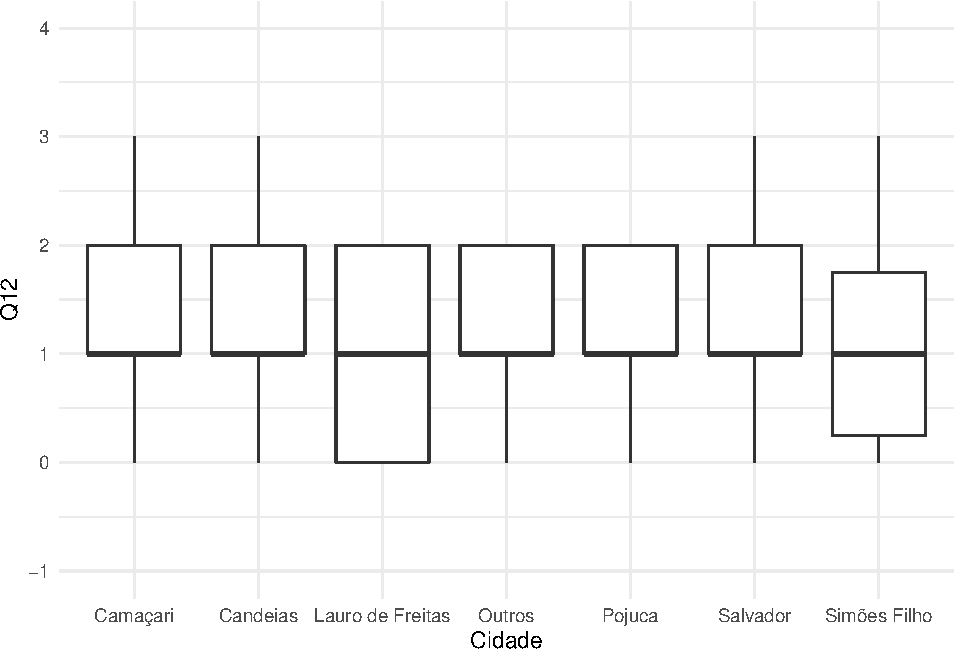
\includegraphics[width=0.75\linewidth]{relatorio_files/figure-latex/unnamed-chunk-21-1} \end{center}

\hypertarget{teste-de-kruskal-wallis-de-q12-por-cidade}{%
\paragraph{Teste de Kruskal-Wallis de Q12 por Cidade}\label{teste-de-kruskal-wallis-de-q12-por-cidade}}

Como o valor-p é menor que \(\alpha=0,05\), não rejeitamos \(H_0\) e as medianas de \(Q12\) entre as crianças de diversas cidades são diferentes.

\begin{longtable}[]{@{}ccc@{}}
\caption{\label{tab:unnamed-chunk-22}Valores-p para comparação múltipla de medianas: Q12 e Cidade.}\tabularnewline
\toprule
Estatística & Parâmetro & valor p\tabularnewline
\midrule
\endfirsthead
\toprule
Estatística & Parâmetro & valor p\tabularnewline
\midrule
\endhead
19,08 & 6 & 0\tabularnewline
\bottomrule
\end{longtable}

\hypertarget{teste-de-nemeyi-de-q12-por-cidade}{%
\paragraph{Teste de Nemeyi de Q12 por Cidade}\label{teste-de-nemeyi-de-q12-por-cidade}}

As medianas de Lauro de Freitas de \emph{Q12} e \emph{Cidade} são diferentes, pois o valor-p \(p = 0,01\) para este par é menor que \(\alpha = 0,05\).

\begin{longtable}[]{@{}lcccccc@{}}
\caption{\label{tab:unnamed-chunk-23}Teste de Nemeyi de Q12 por Cidade.}\tabularnewline
\toprule
& Camaçari & Candeias & Lauro de Freitas & Outros & Pojuca & Salvador\tabularnewline
\midrule
\endfirsthead
\toprule
& Camaçari & Candeias & Lauro de Freitas & Outros & Pojuca & Salvador\tabularnewline
\midrule
\endhead
Candeias & 0,99 & & & & &\tabularnewline
Lauro de Freitas & 0,01 & 0,54 & & & &\tabularnewline
Outros & 0,76 & 1,00 & 0,48 & & &\tabularnewline
Pojuca & 0,99 & 1,00 & 0,27 & 1,00 & &\tabularnewline
Salvador & 0,10 & 1,00 & 0,31 & 1,00 & 0,98 &\tabularnewline
Simões Filho & 0,21 & 0,86 & 1,00 & 0,89 & 0,72 & 0,88\tabularnewline
\bottomrule
\end{longtable}

\cleardoublepage

\hypertarget{tabela-de-continguxeancia-guxeanero-e-q12}{%
\paragraph{Tabela de contingência: Gênero e Q12}\label{tabela-de-continguxeancia-guxeanero-e-q12}}

Apenas seis crianças se identificaram com o gênero \emph{outros} e foram removidas na análise estatística.

\begin{longtable}[]{@{}ccccc@{}}
\caption{\label{tab:unnamed-chunk-24}Tabela de contingência: Gênero e Q12.}\tabularnewline
\toprule
Gênero & Muita preocupação & Pouca preocupação & Sem preocupação & Sem resposta\tabularnewline
\midrule
\endfirsthead
\toprule
Gênero & Muita preocupação & Pouca preocupação & Sem preocupação & Sem resposta\tabularnewline
\midrule
\endhead
Menina & 213 & 214 & 100 & 14\tabularnewline
Menino & 173 & 214 & 103 & 13\tabularnewline
\bottomrule
\end{longtable}

\hypertarget{gruxe1fico-de-barras-guxeanero-e-q12}{%
\paragraph{Gráfico de barras: Gênero e Q12}\label{gruxe1fico-de-barras-guxeanero-e-q12}}

Apenas seis crianças se identificaram com o gênero \emph{outros} e foram removidas na análise estatística.

Aparentemente as duas variáveis \emph{Gênero} e \emph{Q12} não estão associadas.

\begin{center}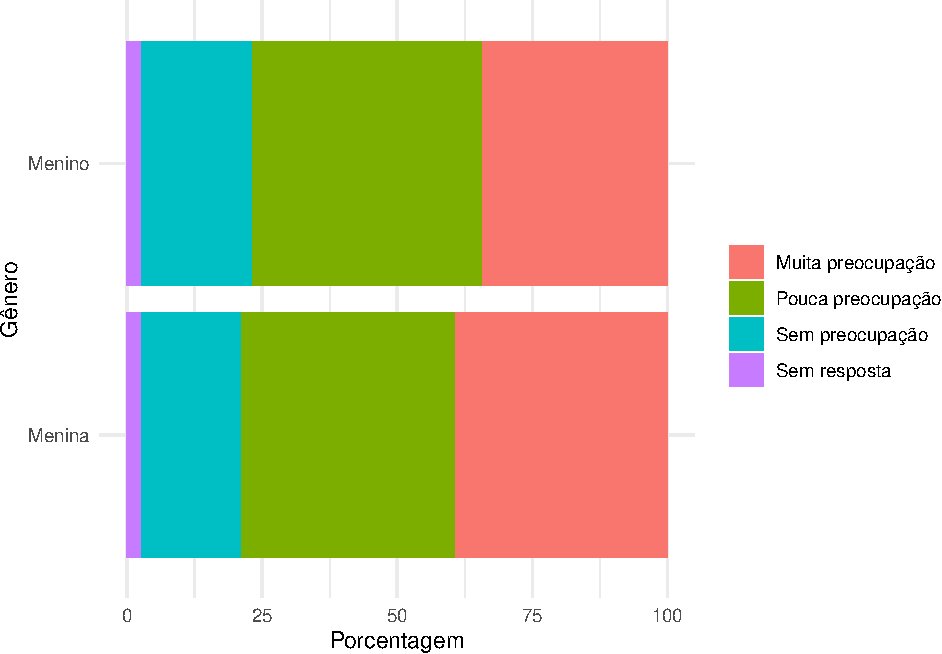
\includegraphics[width=0.75\linewidth]{relatorio_files/figure-latex/unnamed-chunk-25-1} \end{center}

\hypertarget{teste-qui-quadrado-3}{%
\paragraph{Teste qui-quadrado}\label{teste-qui-quadrado-3}}

Apenas seis crianças se identificaram com o gênero \emph{outros} e foram removidas na análise estatística.

Como o valor-p é maior que \(\alpha=0,05\), não rejeitamos \(H_0\) e não temos evidência evidência estatística que as duas variáveis estão associadas.

\begin{longtable}[]{@{}ccc@{}}
\caption{\label{tab:unnamed-chunk-26}Teste qui-quadrado entre Gênero e Q12.}\tabularnewline
\toprule
Estatística & Graus de liberdade & Valor-p\tabularnewline
\midrule
\endfirsthead
\toprule
Estatística & Graus de liberdade & Valor-p\tabularnewline
\midrule
\endhead
2,85 & 3 & 0,42\tabularnewline
\bottomrule
\end{longtable}

\cleardoublepage

\hypertarget{medidas-de-resumo-q12-por-guxeanero}{%
\paragraph{Medidas de Resumo Q12 por Gênero}\label{medidas-de-resumo-q12-por-guxeanero}}

Apenas seis crianças se identificaram com o gênero \emph{outros} e foram removidas na análise estatística.

\begin{longtable}[]{@{}cccccc@{}}
\caption{\label{tab:unnamed-chunk-27}Medidas de resumo de Q12 por Gênero.}\tabularnewline
\toprule
Q12 & Média & Desvio Padrão & Mediana & 1 Quartil & 3 Quartil\tabularnewline
\midrule
\endfirsthead
\toprule
Q12 & Média & Desvio Padrão & Mediana & 1 Quartil & 3 Quartil\tabularnewline
\midrule
\endhead
Menina & 1,26 & 0,78 & 1 & 1 & 2\tabularnewline
Menino & 1,19 & 0,79 & 1 & 1 & 2\tabularnewline
\bottomrule
\end{longtable}

\hypertarget{boxplot-de-q12-por-guxeanero}{%
\paragraph{Boxplot de Q12 por Gênero}\label{boxplot-de-q12-por-guxeanero}}

Apenas seis crianças se identificaram com o gênero \emph{outros} e foram removidas na análise estatística.

\begin{center}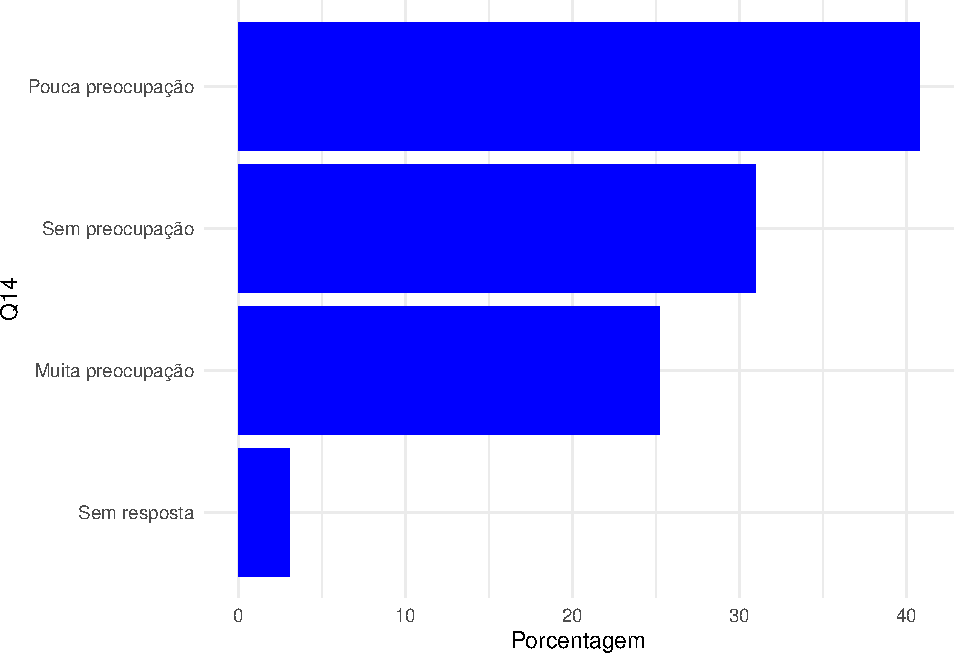
\includegraphics[width=0.75\linewidth]{relatorio_files/figure-latex/unnamed-chunk-28-1} \end{center}

\hypertarget{teste-de-kruskal-wallis-de-q12-por-guxeanero}{%
\paragraph{Teste de Kruskal-Wallis de Q12 por Gênero}\label{teste-de-kruskal-wallis-de-q12-por-guxeanero}}

Apenas seis crianças se identificaram com o gênero \emph{outros} e foram removidas na análise estatística.

Como o valor-p é maior que \(\alpha=0,05\), não rejeitamos \(H_0\) e as medianas de \(Q12\) entre os meninos e as meninas são iguais.

\begin{longtable}[]{@{}ccc@{}}
\caption{\label{tab:unnamed-chunk-29}Valores-p para comparação múltipla de medianas: Q12 e Gênero.}\tabularnewline
\toprule
Estatística & Parâmetro & valor p\tabularnewline
\midrule
\endfirsthead
\toprule
Estatística & Parâmetro & valor p\tabularnewline
\midrule
\endhead
2,31 & 1 & 0,13\tabularnewline
\bottomrule
\end{longtable}

\hypertarget{teste-de-nemeyi-de-q12-por-guxeanero}{%
\paragraph{Teste de Nemeyi de Q12 por Gênero}\label{teste-de-nemeyi-de-q12-por-guxeanero}}

Apenas seis crianças se identificaram com o gênero \emph{outros} e foram removidas na análise estatística.

Como o valor-p é maior que \(\alpha=0,05\), não rejeitamos \(H_0\) e as medianas de \(Q12\) entre os meninos e as meninas são iguais.

\begin{longtable}[]{@{}lc@{}}
\caption{\label{tab:unnamed-chunk-30}Teste de Nemeyi de Q12 por Gênero.}\tabularnewline
\toprule
& Menina\tabularnewline
\midrule
\endfirsthead
\toprule
& Menina\tabularnewline
\midrule
\endhead
Menino & 0,15\tabularnewline
\bottomrule
\end{longtable}

\cleardoublepage

\hypertarget{tabela-de-continguxeancia-idade-e-q12}{%
\paragraph{Tabela de contingência: Idade e Q12}\label{tabela-de-continguxeancia-idade-e-q12}}

\begin{longtable}[]{@{}ccccc@{}}
\caption{\label{tab:unnamed-chunk-31}Tabela de contingência: Idade e Q12.}\tabularnewline
\toprule
Idade & Muita preocupação & Pouca preocupação & Sem preocupação & Sem resposta\tabularnewline
\midrule
\endfirsthead
\toprule
Idade & Muita preocupação & Pouca preocupação & Sem preocupação & Sem resposta\tabularnewline
\midrule
\endhead
8 & 69 & 78 & 41 & 7\tabularnewline
9 & 72 & 82 & 31 & 1\tabularnewline
10 & 101 & 98 & 41 & 10\tabularnewline
11 & 79 & 106 & 50 & 5\tabularnewline
12 & 68 & 66 & 41 & 4\tabularnewline
\bottomrule
\end{longtable}

\hypertarget{gruxe1fico-de-barras-idade-e-q12}{%
\paragraph{Gráfico de barras: Idade e Q12}\label{gruxe1fico-de-barras-idade-e-q12}}

Aparentemente as duas variáveis \emph{Idade} e \emph{Q12} não estão associadas.

\begin{center}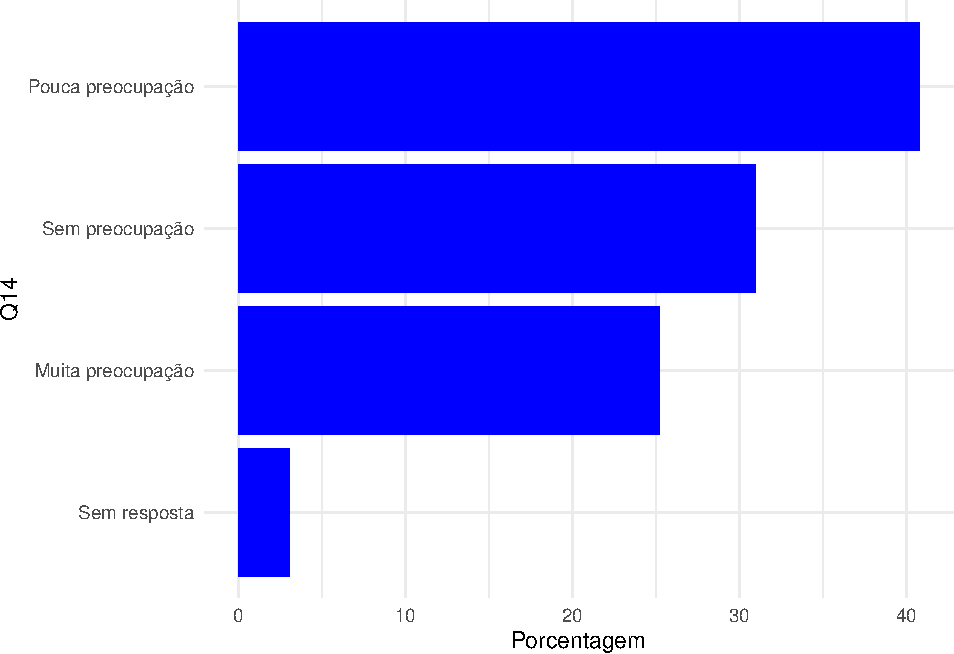
\includegraphics[width=0.75\linewidth]{relatorio_files/figure-latex/unnamed-chunk-32-1} \end{center}

\hypertarget{teste-qui-quadrado-4}{%
\paragraph{Teste qui-quadrado}\label{teste-qui-quadrado-4}}

Como o valor-p é maior que \(\alpha=0,05\), não rejeitamos \(H_0\) e não temos temos evidência evidência estatística que as duas variáveis estão associadas.

\begin{longtable}[]{@{}ccc@{}}
\caption{\label{tab:unnamed-chunk-33}Teste qui-quadrado entre Idade e Q12.}\tabularnewline
\toprule
Estatística & Graus de liberdade & Valor-p\tabularnewline
\midrule
\endfirsthead
\toprule
Estatística & Graus de liberdade & Valor-p\tabularnewline
\midrule
\endhead
13,79 & 12 & 0,31\tabularnewline
\bottomrule
\end{longtable}

\cleardoublepage

\hypertarget{medidas-de-resumo-q12-por-idade}{%
\paragraph{Medidas de Resumo Q12 por Idade}\label{medidas-de-resumo-q12-por-idade}}

\begin{longtable}[]{@{}cccccc@{}}
\caption{\label{tab:unnamed-chunk-34}Medidas de resumo de Q12 por Idade.}\tabularnewline
\toprule
Q12 & Média & Desvio Padrão & Mediana & 1 Quartil & 3 Quartil\tabularnewline
\midrule
\endfirsthead
\toprule
Q12 & Média & Desvio Padrão & Mediana & 1 Quartil & 3 Quartil\tabularnewline
\midrule
\endhead
8 & 1,22 & 0,82 & 1 & 1 & 2\tabularnewline
9 & 1,23 & 0,72 & 1 & 1 & 2\tabularnewline
10 & 1,32 & 0,79 & 1 & 1 & 2\tabularnewline
11 & 1,16 & 0,77 & 1 & 1 & 2\tabularnewline
12 & 1,20 & 0,81 & 1 & 1 & 2\tabularnewline
\bottomrule
\end{longtable}

\hypertarget{boxplot-de-q12-por-idade}{%
\paragraph{Boxplot de Q12 por Idade}\label{boxplot-de-q12-por-idade}}

\begin{center}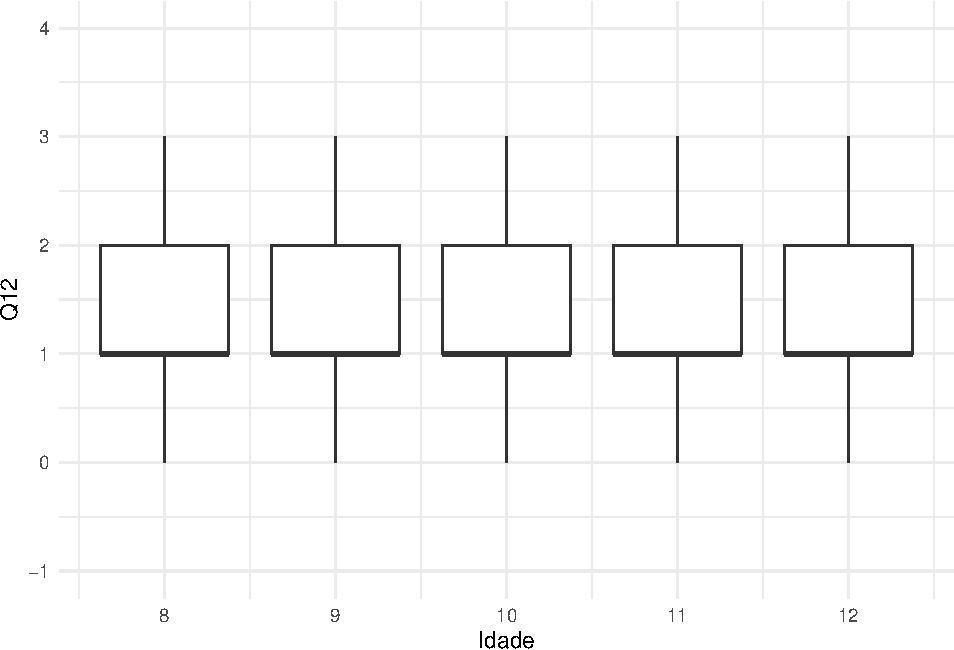
\includegraphics[width=0.75\linewidth]{relatorio_files/figure-latex/unnamed-chunk-35-1} \end{center}

\hypertarget{teste-de-kruskal-wallis-de-q12-por-idade}{%
\paragraph{Teste de Kruskal-Wallis de Q12 por Idade}\label{teste-de-kruskal-wallis-de-q12-por-idade}}

Como o valor-p é maior que \(\alpha=0,05\), não rejeitamos \(H_0\) e as medianas de \(Q12\) de cada idade são iguais.

\begin{longtable}[]{@{}ccc@{}}
\caption{\label{tab:unnamed-chunk-36}Valores-p para comparação múltipla de medianas: Q12 e Idade.}\tabularnewline
\toprule
Estatística & Parâmetro & valor p\tabularnewline
\midrule
\endfirsthead
\toprule
Estatística & Parâmetro & valor p\tabularnewline
\midrule
\endhead
4,11 & 4 & 0,39\tabularnewline
\bottomrule
\end{longtable}

\hypertarget{teste-de-nemeyi-de-q12-por-idade}{%
\paragraph{Teste de Nemeyi de Q12 por Idade}\label{teste-de-nemeyi-de-q12-por-idade}}

Os valores-p são todos maiores que \(\alpha=0,05\), e não rejeitamos \(H_0\) para todos os pares de idade, ou seja, as medianas são iguais para cada par de idade.

\begin{longtable}[]{@{}lcccc@{}}
\caption{\label{tab:unnamed-chunk-37}Teste de Nemeyi de Q12 por Idade.}\tabularnewline
\toprule
& 8 & 9 & 10 & 11\tabularnewline
\midrule
\endfirsthead
\toprule
& 8 & 9 & 10 & 11\tabularnewline
\midrule
\endhead
9 & 1,00 & & &\tabularnewline
10 & 0,69 & 0,86 & &\tabularnewline
11 & 0,97 & 0,89 & 0,24 &\tabularnewline
12 & 1,00 & 1,00 & 0,63 & 0,99\tabularnewline
\bottomrule
\end{longtable}

\cleardoublepage

\hypertarget{tabela-de-continguxeancia-rauxe7a-e-q12}{%
\paragraph{Tabela de contingência: Raça e Q12}\label{tabela-de-continguxeancia-rauxe7a-e-q12}}

\begin{longtable}[]{@{}ccccc@{}}
\caption{\label{tab:unnamed-chunk-38}Tabela de contingência: Raça e Q12.}\tabularnewline
\toprule
Raça & Muita preocupação & Pouca preocupação & Sem preocupação & Sem resposta\tabularnewline
\midrule
\endfirsthead
\toprule
Raça & Muita preocupação & Pouca preocupação & Sem preocupação & Sem resposta\tabularnewline
\midrule
\endhead
Amarela & 8 & 7 & 3 & 1\tabularnewline
Branca & 77 & 86 & 47 & 3\tabularnewline
Indígena & 8 & 10 & 2 & 1\tabularnewline
Negra & 277 & 311 & 140 & 21\tabularnewline
Outros & 8 & 6 & 2 &\tabularnewline
Sem resposta & 11 & 10 & 10 & 1\tabularnewline
\bottomrule
\end{longtable}

\hypertarget{gruxe1fico-de-barras-rauxe7a-e-q12}{%
\paragraph{Gráfico de barras: Raça e Q12}\label{gruxe1fico-de-barras-rauxe7a-e-q12}}

Aparentemente as duas variáveis \emph{Raça} e \emph{Q12} não estão associadas.

\begin{center}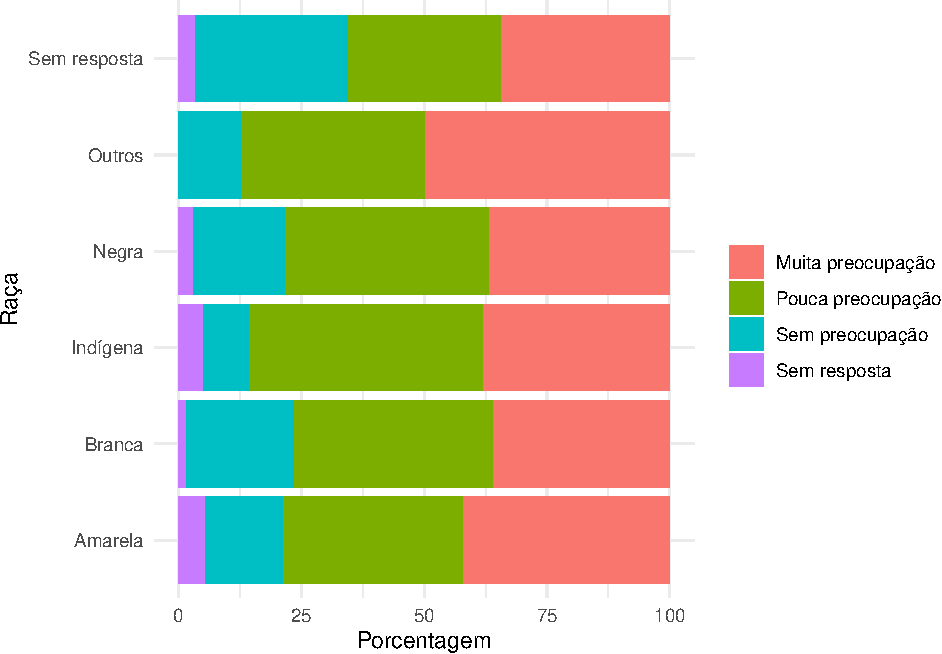
\includegraphics[width=0.75\linewidth]{relatorio_files/figure-latex/unnamed-chunk-39-1} \end{center}

\hypertarget{teste-qui-quadrado-5}{%
\paragraph{Teste qui-quadrado}\label{teste-qui-quadrado-5}}

Como o valor-p é maior que \(\alpha=0,05\), não rejeitamos \(H_0\) e não temos evidência evidência estatística que as duas variáveis estão associadas.

\begin{longtable}[]{@{}ccc@{}}
\caption{\label{tab:unnamed-chunk-40}Teste qui-quadrado entre raca e Q12.}\tabularnewline
\toprule
Estatística & Graus de liberdade & Valor-p\tabularnewline
\midrule
\endfirsthead
\toprule
Estatística & Graus de liberdade & Valor-p\tabularnewline
\midrule
\endhead
9,65 & 15 & 0,84\tabularnewline
\bottomrule
\end{longtable}

\cleardoublepage

\hypertarget{medidas-de-resumo-q12-por-rauxe7a}{%
\paragraph{Medidas de Resumo Q12 por Raça}\label{medidas-de-resumo-q12-por-rauxe7a}}

\begin{longtable}[]{@{}cccccc@{}}
\caption{\label{tab:unnamed-chunk-41}Medidas de resumo de Q12 por raca.}\tabularnewline
\toprule
Q12 & Média & Desvio Padrão & Mediana & 1 Quartil & 3 Quartil\tabularnewline
\midrule
\endfirsthead
\toprule
Q12 & Média & Desvio Padrão & Mediana & 1 Quartil & 3 Quartil\tabularnewline
\midrule
\endhead
Amarela & 1,37 & 0,83 & 1,0 & 1 & 2\tabularnewline
Branca & 1,17 & 0,78 & 1,0 & 1 & 2\tabularnewline
Indígena & 1,38 & 0,74 & 1,0 & 1 & 2\tabularnewline
Negra & 1,24 & 0,78 & 1,0 & 1 & 2\tabularnewline
Outros & 1,38 & 0,72 & 1,5 & 1 & 2\tabularnewline
Sem resposta & 1,09 & 0,89 & 1,0 & 0 & 2\tabularnewline
\bottomrule
\end{longtable}

\hypertarget{boxplot-de-q12-por-rauxe7a}{%
\paragraph{Boxplot de Q12 por Raça}\label{boxplot-de-q12-por-rauxe7a}}

\begin{center}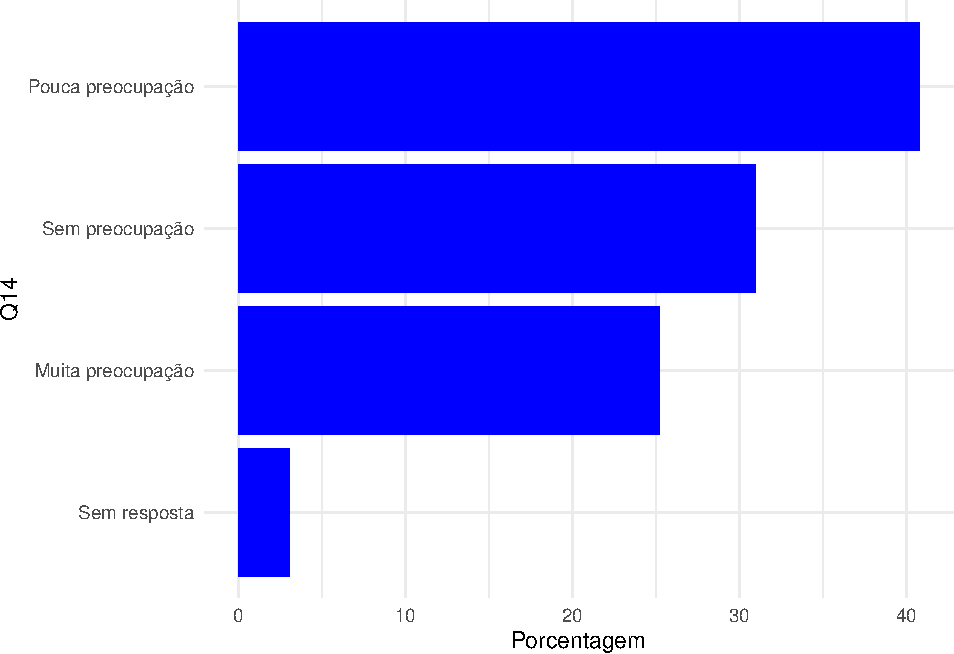
\includegraphics[width=0.75\linewidth]{relatorio_files/figure-latex/unnamed-chunk-42-1} \end{center}

\hypertarget{teste-de-kruskal-wallis-de-q12-por-rauxe7a}{%
\paragraph{Teste de Kruskal-Wallis de Q12 por Raça}\label{teste-de-kruskal-wallis-de-q12-por-rauxe7a}}

Como o valor-p é maior que \(\alpha=0,05\), não rejeitamos \(H_0\) e as medianas de \(Q12\) entre as crianças de diversas raças são iguais.

\begin{longtable}[]{@{}ccc@{}}
\caption{\label{tab:unnamed-chunk-43}Valores-p para comparação múltipla de medianas: Q12 e Raça.}\tabularnewline
\toprule
Estatística & Parâmetro & valor p\tabularnewline
\midrule
\endfirsthead
\toprule
Estatística & Parâmetro & valor p\tabularnewline
\midrule
\endhead
3,8 & 5 & 0,58\tabularnewline
\bottomrule
\end{longtable}

\hypertarget{teste-de-nemeyi-de-q12-por-rauxe7a}{%
\paragraph{Teste de Nemeyi de Q12 por Raça}\label{teste-de-nemeyi-de-q12-por-rauxe7a}}

Como o valor-p é maior que \(\alpha=0,05\), não rejeitamos \(H_0\) e as medianas de \(Q12\) entre as crianças de diversas raças são iguais.

\begin{longtable}[]{@{}lccccc@{}}
\caption{\label{tab:unnamed-chunk-44}Teste de Nemeyi de Q12 por Raça.}\tabularnewline
\toprule
& Amarela & Branca & Indígena & Negra & Outros\tabularnewline
\midrule
\endfirsthead
\toprule
& Amarela & Branca & Indígena & Negra & Outros\tabularnewline
\midrule
\endhead
Branca & 0,94 & & & &\tabularnewline
Indígena & 1,00 & 0,92 & & &\tabularnewline
Negra & 0,99 & 0,93 & 0,98 & &\tabularnewline
Outros & 1,00 & 0,92 & 1,00 & 0,98 &\tabularnewline
Sem resposta & 0,89 & 1,00 & 0,88 & 0,95 & 0,87\tabularnewline
\bottomrule
\end{longtable}

\cleardoublepage

\hypertarget{tabela-de-continguxeancia-tipo-de-escola-e-q12}{%
\paragraph{Tabela de contingência: Tipo de escola e Q12}\label{tabela-de-continguxeancia-tipo-de-escola-e-q12}}

Apenas sete crianças não estavam matriculadas na escola, e foram retiradas da análise para facilitar a análise de \emph{tipo de escola}.

\begin{longtable}[]{@{}ccccc@{}}
\caption{\label{tab:unnamed-chunk-45}Tabela de contingência: Tipo de escola e Q12.}\tabularnewline
\toprule
\begin{minipage}[b]{0.16\columnwidth}\centering
Tipo de Escola\strut
\end{minipage} & \begin{minipage}[b]{0.19\columnwidth}\centering
Muita preocupação\strut
\end{minipage} & \begin{minipage}[b]{0.19\columnwidth}\centering
Pouca preocupação\strut
\end{minipage} & \begin{minipage}[b]{0.17\columnwidth}\centering
Sem preocupação\strut
\end{minipage} & \begin{minipage}[b]{0.14\columnwidth}\centering
Sem resposta\strut
\end{minipage}\tabularnewline
\midrule
\endfirsthead
\toprule
\begin{minipage}[b]{0.16\columnwidth}\centering
Tipo de Escola\strut
\end{minipage} & \begin{minipage}[b]{0.19\columnwidth}\centering
Muita preocupação\strut
\end{minipage} & \begin{minipage}[b]{0.19\columnwidth}\centering
Pouca preocupação\strut
\end{minipage} & \begin{minipage}[b]{0.17\columnwidth}\centering
Sem preocupação\strut
\end{minipage} & \begin{minipage}[b]{0.14\columnwidth}\centering
Sem resposta\strut
\end{minipage}\tabularnewline
\midrule
\endhead
\begin{minipage}[t]{0.16\columnwidth}\centering
Particular\strut
\end{minipage} & \begin{minipage}[t]{0.19\columnwidth}\centering
199\strut
\end{minipage} & \begin{minipage}[t]{0.19\columnwidth}\centering
240\strut
\end{minipage} & \begin{minipage}[t]{0.17\columnwidth}\centering
139\strut
\end{minipage} & \begin{minipage}[t]{0.14\columnwidth}\centering
12\strut
\end{minipage}\tabularnewline
\begin{minipage}[t]{0.16\columnwidth}\centering
Pública\strut
\end{minipage} & \begin{minipage}[t]{0.19\columnwidth}\centering
190\strut
\end{minipage} & \begin{minipage}[t]{0.19\columnwidth}\centering
187\strut
\end{minipage} & \begin{minipage}[t]{0.17\columnwidth}\centering
61\strut
\end{minipage} & \begin{minipage}[t]{0.14\columnwidth}\centering
15\strut
\end{minipage}\tabularnewline
\bottomrule
\end{longtable}

\hypertarget{gruxe1fico-de-barras-tipo-de-escola-e-q12}{%
\paragraph{Gráfico de barras: Tipo de escola e Q12}\label{gruxe1fico-de-barras-tipo-de-escola-e-q12}}

Apenas sete crianças não estavam matriculadas na escola, e foram retiradas da análise para facilitar a análise de \emph{tipo de escola}.

Aparentemente as duas variáveis \emph{Tipo de Escola} e \emph{Q12} não estão associadas.

\begin{center}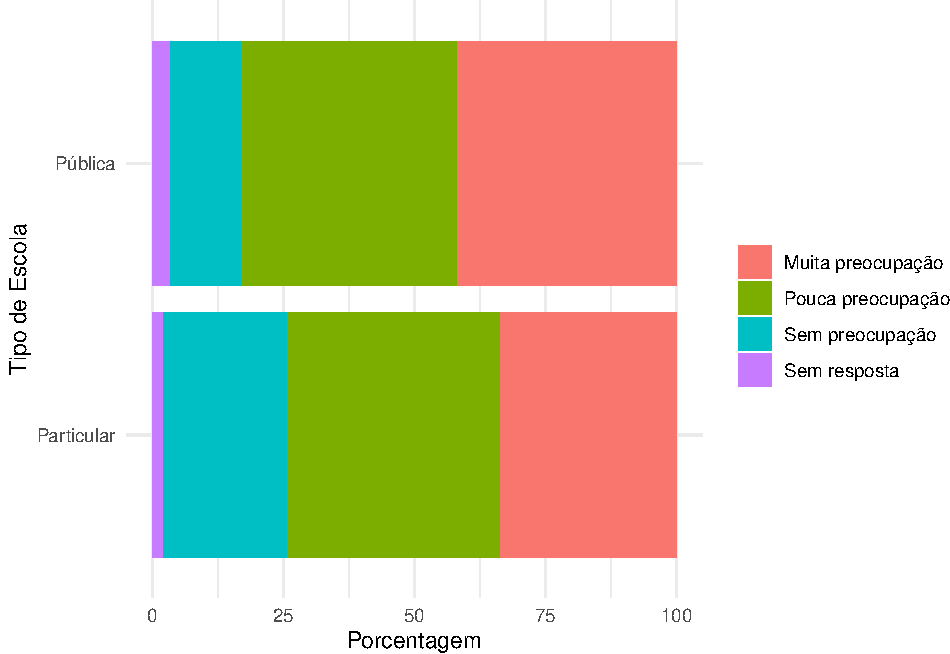
\includegraphics[width=0.75\linewidth]{relatorio_files/figure-latex/unnamed-chunk-46-1} \end{center}

\hypertarget{teste-qui-quadrado-6}{%
\paragraph{Teste qui-quadrado}\label{teste-qui-quadrado-6}}

Apenas sete crianças não estavam matriculadas na escola, e foram retiradas da análise para facilitar a análise de \emph{tipo de escola}.

Como o valor-p é menor que \(\alpha=0,05\), rejeitamos \(H_0\) e temos evidência evidência estatística que as duas variáveis estão associadas.

\begin{longtable}[]{@{}ccc@{}}
\caption{\label{tab:unnamed-chunk-47}Teste qui-quadrado entre Escola e Q12.}\tabularnewline
\toprule
Estatística & Graus de liberdade & Valor-p\tabularnewline
\midrule
\endfirsthead
\toprule
Estatística & Graus de liberdade & Valor-p\tabularnewline
\midrule
\endhead
19,89 & 3 & 0\tabularnewline
\bottomrule
\end{longtable}

\cleardoublepage

\hypertarget{medidas-de-resumo-q12-por-tipo-de-escola}{%
\paragraph{Medidas de Resumo Q12 por Tipo de escola}\label{medidas-de-resumo-q12-por-tipo-de-escola}}

Apenas sete crianças não estavam matriculadas na escola, e foram retiradas da análise para facilitar a análise de \emph{tipo de escola}.

\begin{longtable}[]{@{}cccccc@{}}
\caption{\label{tab:unnamed-chunk-48}Medidas de resumo de Q12 por Escola.}\tabularnewline
\toprule
Q12 & Média & Desvio Padrão & Mediana & 1 Quartil & 3 Quartil\tabularnewline
\midrule
\endfirsthead
\toprule
Q12 & Média & Desvio Padrão & Mediana & 1 Quartil & 3 Quartil\tabularnewline
\midrule
\endhead
Particular & 1,14 & 0,80 & 1 & 1 & 2\tabularnewline
Pública & 1,35 & 0,75 & 1 & 1 & 2\tabularnewline
\bottomrule
\end{longtable}

\hypertarget{boxplot-de-q12-por-tipo-de-escola}{%
\paragraph{Boxplot de Q12 por Tipo de escola}\label{boxplot-de-q12-por-tipo-de-escola}}

Apenas sete crianças não estavam matriculadas na escola, e foram retiradas da análise para facilitar a análise de \emph{tipo de escola}.

\begin{center}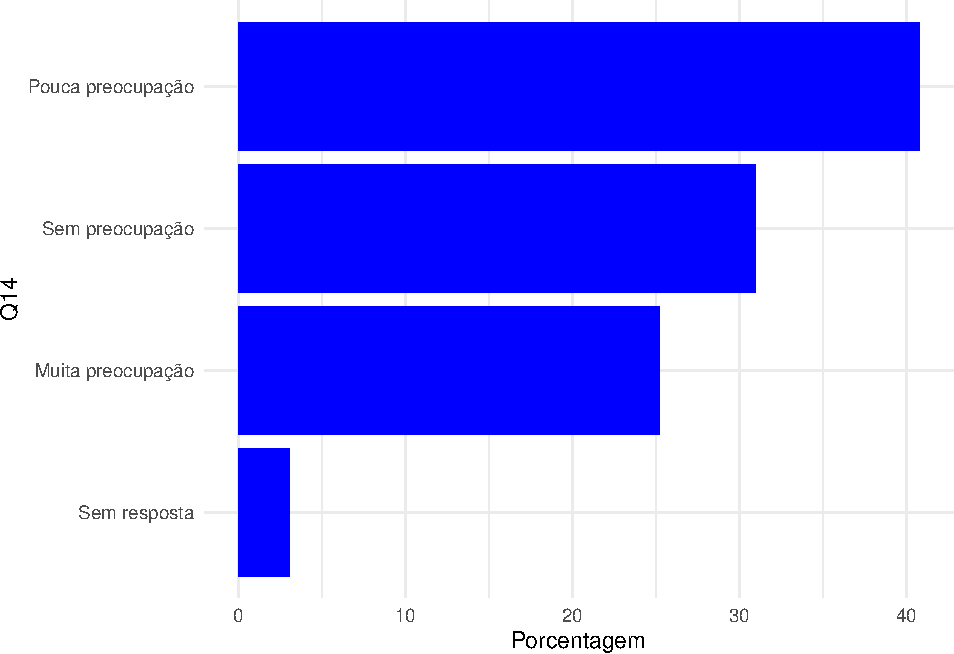
\includegraphics[width=0.75\linewidth]{relatorio_files/figure-latex/unnamed-chunk-49-1} \end{center}

\hypertarget{teste-de-kruskal-wallis-de-q12-por-tipo-de-escola}{%
\paragraph{Teste de Kruskal-Wallis de Q12 por Tipo de escola}\label{teste-de-kruskal-wallis-de-q12-por-tipo-de-escola}}

Apenas sete crianças não estavam matriculadas na escola, e foram retiradas da análise para facilitar a análise de \emph{tipo de escola}.

Como o valor-p é menor que \(\alpha=0,05\), rejeitamos \(H_0\) e as medianas de \(Q12\) entre as escolas particulares e públicas são diferentes.

\begin{longtable}[]{@{}ccc@{}}
\caption{\label{tab:unnamed-chunk-50}Valores-p para comparação múltipla de medianas: Q12 e Tipo de escola.}\tabularnewline
\toprule
Estatística & Parâmetro & valor p\tabularnewline
\midrule
\endfirsthead
\toprule
Estatística & Parâmetro & valor p\tabularnewline
\midrule
\endhead
11,54 & 1 & 0\tabularnewline
\bottomrule
\end{longtable}

\hypertarget{teste-de-nemeyi-de-q12-por-tipo-de-escola}{%
\paragraph{Teste de Nemeyi de Q12 por Tipo de escola}\label{teste-de-nemeyi-de-q12-por-tipo-de-escola}}

Apenas sete crianças não estavam matriculadas na escola, e foram retiradas da análise para facilitar a análise de \emph{tipo de escola}.

Como o valor-p é menor que \(\alpha=0,05\), rejeitamos \(H_0\) e as medianas de \(Q12\) entre as escolas particulares e públicas são diferentes.

\begin{longtable}[]{@{}lc@{}}
\caption{\label{tab:unnamed-chunk-51}Teste de Nemeyi de Q12 por Escola.}\tabularnewline
\toprule
& Particular\tabularnewline
\midrule
\endfirsthead
\toprule
& Particular\tabularnewline
\midrule
\endhead
Pública & 0\tabularnewline
\bottomrule
\end{longtable}

\cleardoublepage

\hypertarget{anuxe1lise-descritiva-para-q13}{%
\subsubsection{Análise descritiva para Q13}\label{anuxe1lise-descritiva-para-q13}}

\hypertarget{gruxe1fico-de-barras-q13}{%
\paragraph{Gráfico de barras: Q13}\label{gruxe1fico-de-barras-q13}}

\begin{center}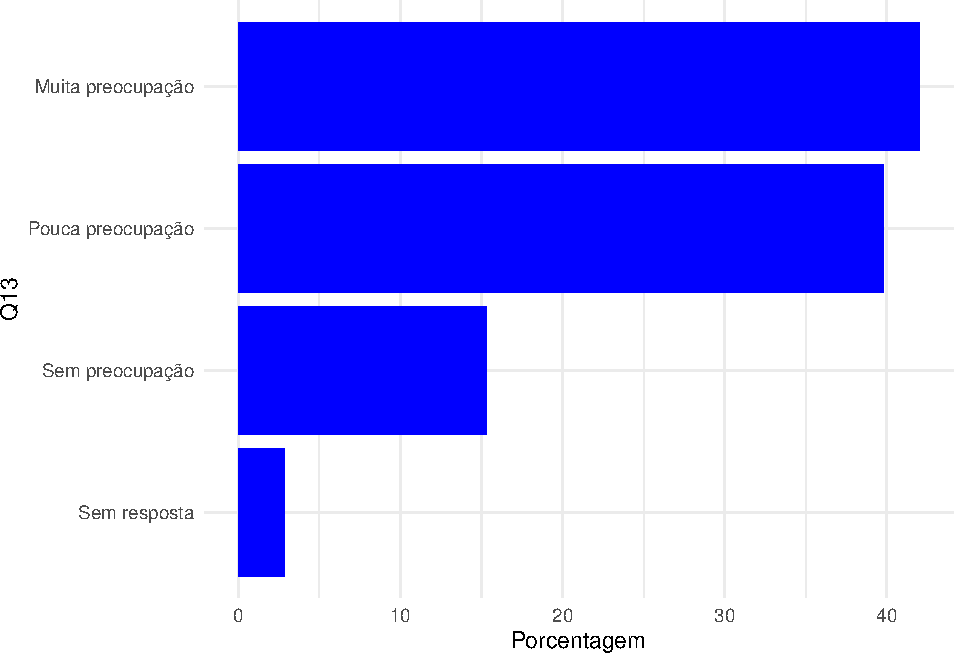
\includegraphics[width=0.75\linewidth]{relatorio_files/figure-latex/unnamed-chunk-52-1} \end{center}

\hypertarget{tabela-de-distribuiuxe7uxe3o-q12-1}{%
\paragraph{Tabela de distribuição: Q12}\label{tabela-de-distribuiuxe7uxe3o-q12-1}}

\begin{longtable}[]{@{}cccc@{}}
\caption{\label{tab:unnamed-chunk-53}Que demorasse muito para eu encontrar meus amigos?}\tabularnewline
\toprule
Q13 & Frequência & Frequência relativa & Porcentagem\tabularnewline
\midrule
\endfirsthead
\toprule
Q13 & Frequência & Frequência relativa & Porcentagem\tabularnewline
\midrule
\endhead
Muita preocupação & 441 & 0,42 & 42,00\tabularnewline
Pouca preocupação & 418 & 0,40 & 39,81\tabularnewline
Sem preocupação & 161 & 0,15 & 15,33\tabularnewline
Sem resposta & 30 & 0,03 & 2,86\tabularnewline
\bottomrule
\end{longtable}

\hypertarget{medidas-de-resumo-q12-1}{%
\paragraph{Medidas de resumo: Q12}\label{medidas-de-resumo-q12-1}}

\begin{longtable}[]{@{}ccccc@{}}
\caption{\label{tab:unnamed-chunk-54}Resumos para variável Q13.}\tabularnewline
\toprule
Média & Desvio Padrão & Mediana & 1Qua & 3Qua\tabularnewline
\midrule
\endfirsthead
\toprule
Média & Desvio Padrão & Mediana & 1Qua & 3Qua\tabularnewline
\midrule
\endhead
1,32 & 0,76 & 1 & 1 & 2\tabularnewline
\bottomrule
\end{longtable}

\cleardoublepage

\hypertarget{anuxe1lise-bidimensional-para-q13}{%
\subsubsection{Análise bidimensional para Q13}\label{anuxe1lise-bidimensional-para-q13}}

\hypertarget{tabela-de-continguxeancia-cidade-e-q13}{%
\paragraph{Tabela de contingência: Cidade e Q13}\label{tabela-de-continguxeancia-cidade-e-q13}}

\begin{longtable}[]{@{}ccccc@{}}
\caption{\label{tab:unnamed-chunk-55}Tabela de contingência: Cidade e Q13.}\tabularnewline
\toprule
Cidade & Muita preocupação & Pouca preocupação & Sem preocupação & Sem resposta\tabularnewline
\midrule
\endfirsthead
\toprule
Cidade & Muita preocupação & Pouca preocupação & Sem preocupação & Sem resposta\tabularnewline
\midrule
\endhead
Camaçari & 81 & 79 & 27 & 10\tabularnewline
Candeias & 19 & 14 & 5 &\tabularnewline
Lauro de Freitas & 21 & 28 & 12 &\tabularnewline
Outros & 35 & 32 & 16 &\tabularnewline
Pojuca & 23 & 31 & 8 & 2\tabularnewline
Salvador & 249 & 223 & 84 & 17\tabularnewline
Simões Filho & 13 & 11 & 9 & 1\tabularnewline
\bottomrule
\end{longtable}

\hypertarget{gruxe1fico-de-barras-cidade-e-q13}{%
\paragraph{Gráfico de barras: Cidade e Q13}\label{gruxe1fico-de-barras-cidade-e-q13}}

Aparentemente as duas variáveis \emph{Cidade} e \emph{Q13} não estão associadas.

\begin{center}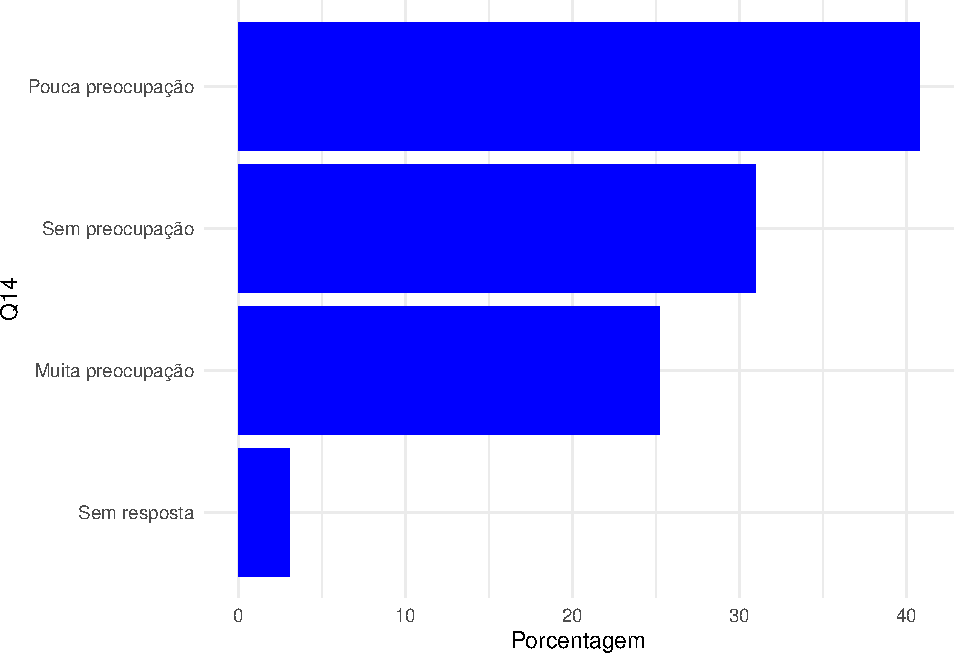
\includegraphics[width=0.75\linewidth]{relatorio_files/figure-latex/unnamed-chunk-56-1} \end{center}

\hypertarget{teste-qui-quadrado-7}{%
\paragraph{Teste qui-quadrado}\label{teste-qui-quadrado-7}}

Como o valor-p é maior que \(\alpha=0,05\), não rejeitamos \(H_0\) e não temos evidência evidência estatística que as duas variáveis estão associadas.

\begin{longtable}[]{@{}ccc@{}}
\caption{\label{tab:unnamed-chunk-57}Teste qui-quadrado entre Cidade e Q13.}\tabularnewline
\toprule
Estatística & Graus de liberdade & Valor-p\tabularnewline
\midrule
\endfirsthead
\toprule
Estatística & Graus de liberdade & Valor-p\tabularnewline
\midrule
\endhead
18,83 & 18 & 0,4\tabularnewline
\bottomrule
\end{longtable}

\cleardoublepage

\hypertarget{medidas-de-resumo-q13-por-cidade}{%
\paragraph{Medidas de Resumo Q13 por Cidade}\label{medidas-de-resumo-q13-por-cidade}}

\begin{longtable}[]{@{}cccccc@{}}
\caption{\label{tab:unnamed-chunk-58}Medidas de resumo de Q13 por Cidade.}\tabularnewline
\toprule
Q13 & Média & Desvio Padrão & Mediana & 1 Quartil & 3 Quartil\tabularnewline
\midrule
\endfirsthead
\toprule
Q13 & Média & Desvio Padrão & Mediana & 1 Quartil & 3 Quartil\tabularnewline
\midrule
\endhead
Camaçari & 1,38 & 0,78 & 1,0 & 1,00 & 2\tabularnewline
Candeias & 1,37 & 0,71 & 1,5 & 1,00 & 2\tabularnewline
Lauro de Freitas & 1,15 & 0,73 & 1,0 & 1,00 & 2\tabularnewline
Outros & 1,23 & 0,75 & 1,0 & 1,00 & 2\tabularnewline
Pojuca & 1,30 & 0,73 & 1,0 & 1,00 & 2\tabularnewline
Salvador & 1,35 & 0,76 & 1,0 & 1,00 & 2\tabularnewline
Simões Filho & 1,18 & 0,87 & 1,0 & 0,25 & 2\tabularnewline
\bottomrule
\end{longtable}

\hypertarget{boxplot-de-q13-por-cidade}{%
\paragraph{Boxplot de Q13 por Cidade}\label{boxplot-de-q13-por-cidade}}

\begin{center}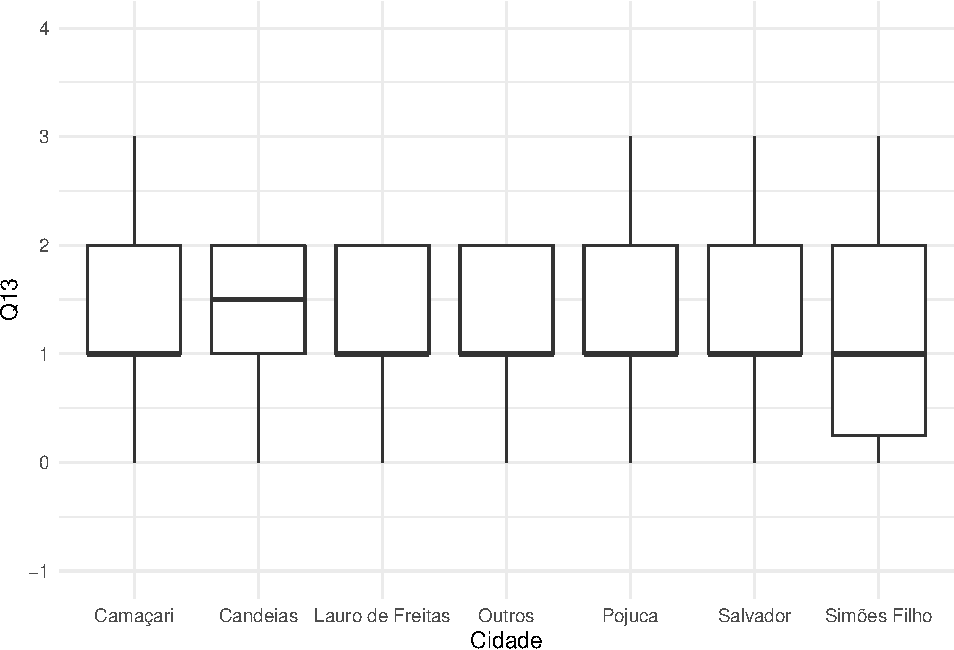
\includegraphics[width=0.75\linewidth]{relatorio_files/figure-latex/unnamed-chunk-59-1} \end{center}

\hypertarget{teste-de-kruskal-wallis-de-q13-por-cidade}{%
\paragraph{Teste de Kruskal-Wallis de Q13 por Cidade}\label{teste-de-kruskal-wallis-de-q13-por-cidade}}

Como o valor-p é maior que \(\alpha=0,05\), não rejeitamos \(H_0\) e as medianas de \(Q13\) entre as crianças de diversas cidades são iguais.

\begin{longtable}[]{@{}ccc@{}}
\caption{\label{tab:unnamed-chunk-60}Valores-p para comparação múltipla de medianas: Q13 e Cidade.}\tabularnewline
\toprule
Estatística & Parâmetro & valor p\tabularnewline
\midrule
\endfirsthead
\toprule
Estatística & Parâmetro & valor p\tabularnewline
\midrule
\endhead
6,71 & 6 & 0,35\tabularnewline
\bottomrule
\end{longtable}

\hypertarget{teste-de-nemeyi-de-q13-por-cidade}{%
\paragraph{Teste de Nemeyi de Q13 por Cidade}\label{teste-de-nemeyi-de-q13-por-cidade}}

Como os valores-p são maiores que \(\alpha=0,05\), não rejeitamos \(H_0\) e as medianas de \(Q12\) entre as crianças de diversas cidades são iguais.

\begin{longtable}[]{@{}lccccc@{}}
\caption{\label{tab:unnamed-chunk-61}Teste de Nemeyi de Q13 por Cidade.}\tabularnewline
\toprule
& Amarela & Branca & Indígena & Negra & Outros\tabularnewline
\midrule
\endfirsthead
\toprule
& Amarela & Branca & Indígena & Negra & Outros\tabularnewline
\midrule
\endhead
Branca & 1,00 & & & &\tabularnewline
Indígena & 1,00 & 1,00 & & &\tabularnewline
Negra & 1,00 & 1,00 & 1,00 & &\tabularnewline
Outros & 0,98 & 0,89 & 0,96 & 0,93 &\tabularnewline
Sem resposta & 0,98 & 0,95 & 0,99 & 0,88 & 0,69\tabularnewline
\bottomrule
\end{longtable}

\cleardoublepage

\hypertarget{tabela-de-continguxeancia-guxeanero-e-q13}{%
\paragraph{Tabela de contingência: Gênero e Q13}\label{tabela-de-continguxeancia-guxeanero-e-q13}}

Apenas seis crianças se identificaram com o gênero \emph{outros} e foram removidas na análise estatística.

\begin{longtable}[]{@{}ccccc@{}}
\caption{\label{tab:unnamed-chunk-62}Tabela de contingência: Gênero e Q13.}\tabularnewline
\toprule
Gênero & Muita preocupação & Pouca preocupação & Sem preocupação & Sem resposta\tabularnewline
\midrule
\endfirsthead
\toprule
Gênero & Muita preocupação & Pouca preocupação & Sem preocupação & Sem resposta\tabularnewline
\midrule
\endhead
Menina & 226 & 210 & 87 & 18\tabularnewline
Menino & 212 & 208 & 72 & 11\tabularnewline
\bottomrule
\end{longtable}

\hypertarget{gruxe1fico-de-barras-guxeanero-e-q13}{%
\paragraph{Gráfico de barras: Gênero e Q13}\label{gruxe1fico-de-barras-guxeanero-e-q13}}

Apenas seis crianças se identificaram com o gênero \emph{outros} e foram removidas na análise estatística.

Aparentemente as duas variáveis \emph{Gênero} e \emph{Q13} não estão associadas.

\begin{center}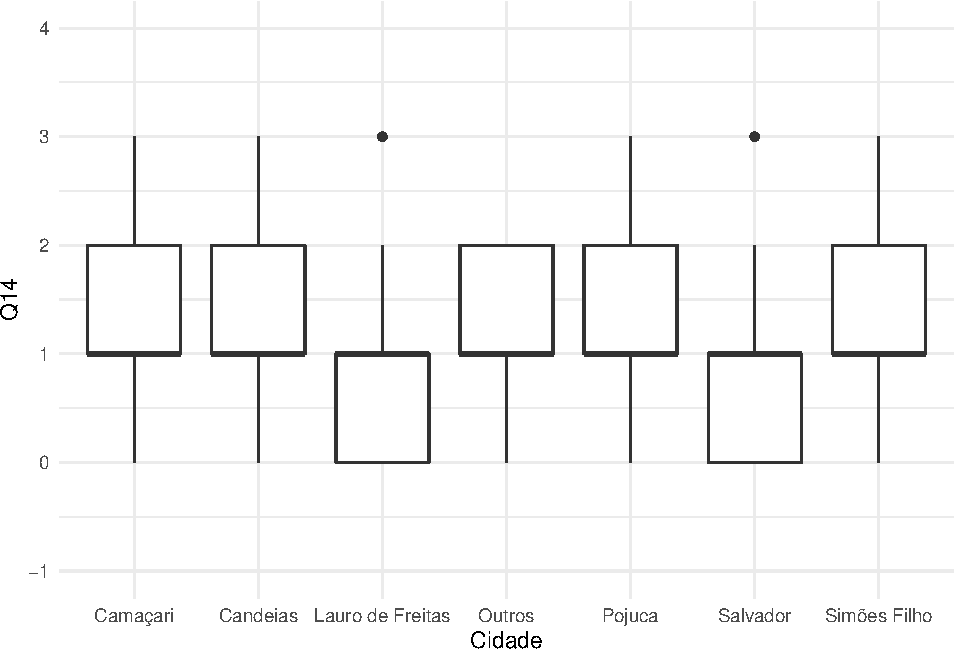
\includegraphics[width=0.75\linewidth]{relatorio_files/figure-latex/unnamed-chunk-63-1} \end{center}

\hypertarget{teste-qui-quadrado-8}{%
\paragraph{Teste qui-quadrado}\label{teste-qui-quadrado-8}}

Apenas seis crianças se identificaram com o gênero \emph{outros} e foram removidas na análise estatística.

Como o valor-p é maior que \(\alpha=0,05\), não rejeitamos \(H_0\) e não temos evidência evidência estatística que as duas variáveis estão associadas.

\begin{longtable}[]{@{}ccc@{}}
\caption{\label{tab:unnamed-chunk-64}Teste qui-quadrado entre Gênero e Q13.}\tabularnewline
\toprule
Estatística & Graus de liberdade & Valor-p\tabularnewline
\midrule
\endfirsthead
\toprule
Estatística & Graus de liberdade & Valor-p\tabularnewline
\midrule
\endhead
2,18 & 3 & 0,54\tabularnewline
\bottomrule
\end{longtable}

\cleardoublepage

\hypertarget{medidas-de-resumo-q13-por-guxeanero}{%
\paragraph{Medidas de Resumo Q13 por Gênero}\label{medidas-de-resumo-q13-por-guxeanero}}

Apenas seis crianças se identificaram com o gênero \emph{outros} e foram removidas na análise estatística.

\begin{longtable}[]{@{}cccccc@{}}
\caption{\label{tab:unnamed-chunk-65}Medidas de resumo de Q13 por Gênero.}\tabularnewline
\toprule
Q13 & Média & Desvio Padrão & Mediana & 1 Quartil & 3 Quartil\tabularnewline
\midrule
\endfirsthead
\toprule
Q13 & Média & Desvio Padrão & Mediana & 1 Quartil & 3 Quartil\tabularnewline
\midrule
\endhead
Menina & 1,32 & 0,78 & 1 & 1 & 2\tabularnewline
Menino & 1,32 & 0,74 & 1 & 1 & 2\tabularnewline
\bottomrule
\end{longtable}

\hypertarget{boxplot-de-q13-por-guxeanero}{%
\paragraph{Boxplot de Q13 por Gênero}\label{boxplot-de-q13-por-guxeanero}}

Apenas seis crianças se identificaram com o gênero \emph{outros} e foram removidas na análise estatística.

\begin{center}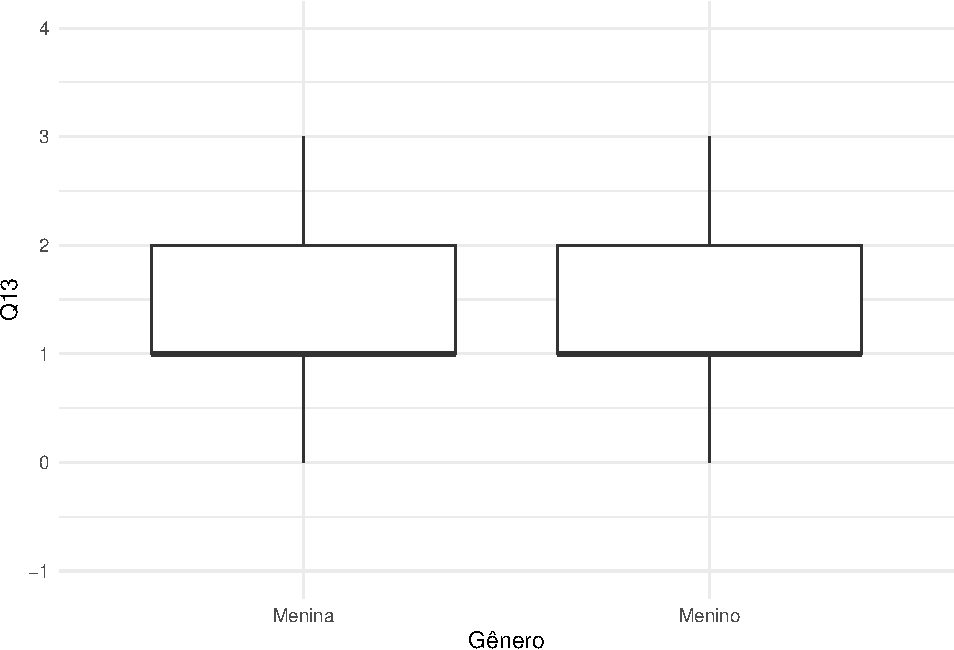
\includegraphics[width=0.75\linewidth]{relatorio_files/figure-latex/unnamed-chunk-66-1} \end{center}

\hypertarget{teste-de-kruskal-wallis-de-q13-por-guxeanero}{%
\paragraph{Teste de Kruskal-Wallis de Q13 por Gênero}\label{teste-de-kruskal-wallis-de-q13-por-guxeanero}}

Apenas seis crianças se identificaram com o gênero \emph{outros} e foram removidas na análise estatística.

Como o valor-p é maior que \(\alpha=0,05\), não rejeitamos \(H_0\) e as medianas de \(Q12\) entre os meninos e as meninas são iguais.

\begin{longtable}[]{@{}ccc@{}}
\caption{\label{tab:unnamed-chunk-67}Valores-p para comparação múltipla de medianas: Q13 e Gênero.}\tabularnewline
\toprule
Estatística & Parâmetro & valor p\tabularnewline
\midrule
\endfirsthead
\toprule
Estatística & Parâmetro & valor p\tabularnewline
\midrule
\endhead
0,41 & 1 & 0,52\tabularnewline
\bottomrule
\end{longtable}

\hypertarget{teste-de-nemeyi-de-q13-por-guxeanero}{%
\paragraph{Teste de Nemeyi de Q13 por Gênero}\label{teste-de-nemeyi-de-q13-por-guxeanero}}

Apenas seis crianças se identificaram com o gênero \emph{outros} e foram removidas na análise estatística.

Como o valor-p é maior que \(\alpha=0,05\), não rejeitamos \(H_0\) e as medianas de \(Q12\) entre os meninos e as meninas são iguais.

\begin{longtable}[]{@{}lc@{}}
\caption{\label{tab:unnamed-chunk-68}Teste de Nemeyi de Q13 por Gênero.}\tabularnewline
\toprule
& Menina\tabularnewline
\midrule
\endfirsthead
\toprule
& Menina\tabularnewline
\midrule
\endhead
Menino & 0,96\tabularnewline
\bottomrule
\end{longtable}

\cleardoublepage

\hypertarget{tabela-de-continguxeancia-idade-e-q13}{%
\paragraph{Tabela de contingência: Idade e Q13}\label{tabela-de-continguxeancia-idade-e-q13}}

\begin{longtable}[]{@{}ccccc@{}}
\caption{\label{tab:unnamed-chunk-69}Tabela de contingência: Idade e Q13.}\tabularnewline
\toprule
Idade & Muita preocupação & Pouca preocupação & Sem preocupação & Sem resposta\tabularnewline
\midrule
\endfirsthead
\toprule
Idade & Muita preocupação & Pouca preocupação & Sem preocupação & Sem resposta\tabularnewline
\midrule
\endhead
8 & 77 & 81 & 27 & 10\tabularnewline
9 & 89 & 65 & 29 & 3\tabularnewline
10 & 107 & 96 & 36 & 11\tabularnewline
11 & 91 & 110 & 34 & 5\tabularnewline
12 & 77 & 66 & 35 & 1\tabularnewline
\bottomrule
\end{longtable}

\hypertarget{gruxe1fico-de-barras-idade-e-q13}{%
\paragraph{Gráfico de barras: Idade e Q13}\label{gruxe1fico-de-barras-idade-e-q13}}

Aparentemente as duas variáveis \emph{Idade} e \emph{Q13} não estão associadas.

\begin{center}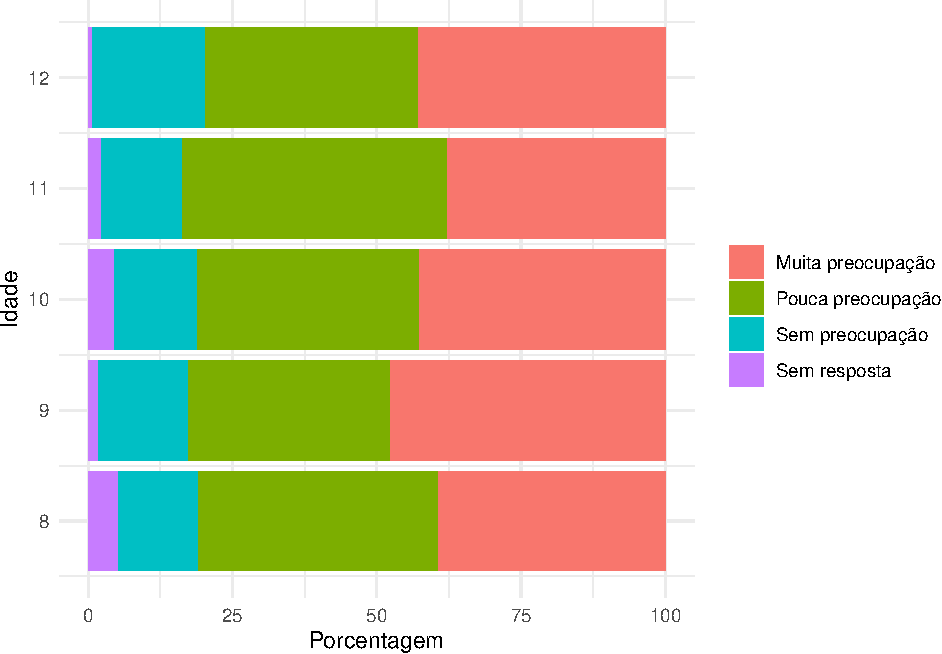
\includegraphics[width=0.75\linewidth]{relatorio_files/figure-latex/unnamed-chunk-70-1} \end{center}

\hypertarget{teste-qui-quadrado-9}{%
\paragraph{Teste qui-quadrado}\label{teste-qui-quadrado-9}}

Como o valor-p é maior que \(\alpha=0,05\), não rejeitamos \(H_0\) e não temos temos evidência evidência estatística que as duas variáveis estão associadas.

\begin{longtable}[]{@{}ccc@{}}
\caption{\label{tab:unnamed-chunk-71}Teste qui-quadrado entre Idade e Q13.}\tabularnewline
\toprule
Estatística & Graus de liberdade & Valor-p\tabularnewline
\midrule
\endfirsthead
\toprule
Estatística & Graus de liberdade & Valor-p\tabularnewline
\midrule
\endhead
19,94 & 12 & 0,07\tabularnewline
\bottomrule
\end{longtable}

\cleardoublepage

\hypertarget{medidas-de-resumo-q13-por-idade}{%
\paragraph{Medidas de Resumo Q13 por Idade}\label{medidas-de-resumo-q13-por-idade}}

\begin{longtable}[]{@{}cccccc@{}}
\caption{\label{tab:unnamed-chunk-72}Medidas de resumo de Q13 por Idade.}\tabularnewline
\toprule
Q13 & Média & Desvio Padrão & Mediana & 1 Quartil & 3 Quartil\tabularnewline
\midrule
\endfirsthead
\toprule
Q13 & Média & Desvio Padrão & Mediana & 1 Quartil & 3 Quartil\tabularnewline
\midrule
\endhead
8 & 1,36 & 0,78 & 1 & 1 & 2\tabularnewline
9 & 1,35 & 0,76 & 1 & 1 & 2\tabularnewline
10 & 1,37 & 0,78 & 1 & 1 & 2\tabularnewline
11 & 1,28 & 0,73 & 1 & 1 & 2\tabularnewline
12 & 1,25 & 0,77 & 1 & 1 & 2\tabularnewline
\bottomrule
\end{longtable}

\hypertarget{boxplot-de-q13-por-idade}{%
\paragraph{Boxplot de Q13 por Idade}\label{boxplot-de-q13-por-idade}}

\begin{center}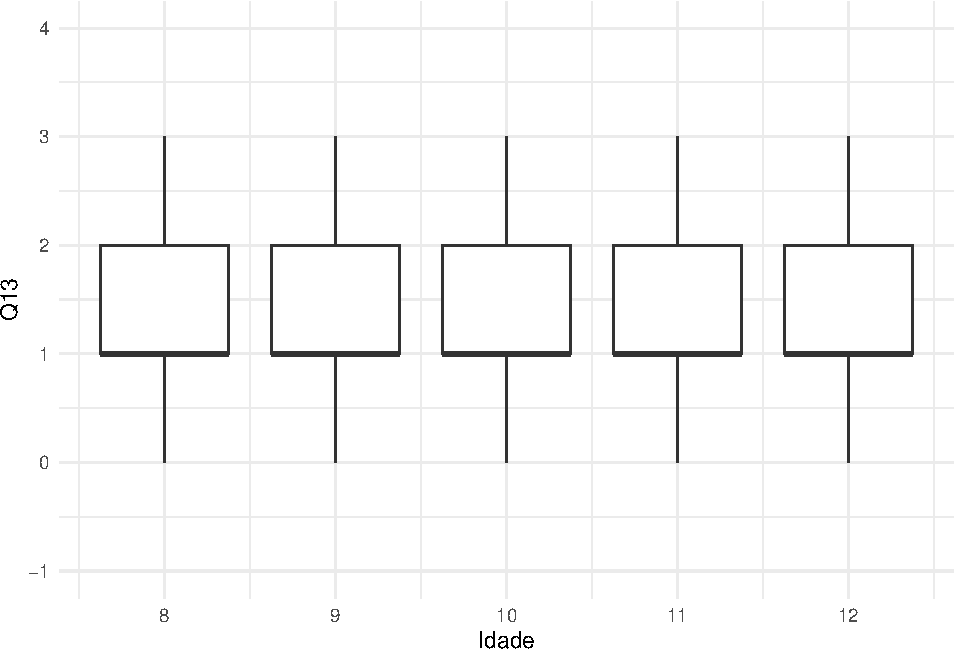
\includegraphics[width=0.75\linewidth]{relatorio_files/figure-latex/unnamed-chunk-73-1} \end{center}

\hypertarget{teste-de-kruskal-wallis-de-q13-por-idade}{%
\paragraph{Teste de Kruskal-Wallis de Q13 por Idade}\label{teste-de-kruskal-wallis-de-q13-por-idade}}

Como o valor-p é maior que \(\alpha=0,05\), não rejeitamos \(H_0\) e as medianas de \(Q13\) de cada idade são iguais.

\begin{longtable}[]{@{}ccc@{}}
\caption{\label{tab:unnamed-chunk-74}Valores-p para comparação múltipla de medianas: Q13 e Idade.}\tabularnewline
\toprule
Estatística & Parâmetro & valor p\tabularnewline
\midrule
\endfirsthead
\toprule
Estatística & Parâmetro & valor p\tabularnewline
\midrule
\endhead
2,96 & 4 & 0,57\tabularnewline
\bottomrule
\end{longtable}

\hypertarget{teste-de-nemeyi-de-q13-por-idade}{%
\paragraph{Teste de Nemeyi de Q13 por Idade}\label{teste-de-nemeyi-de-q13-por-idade}}

Os valores-p são todos maiores que \(\alpha=0,05\), e não rejeitamos \(H_0\) para todos os pares de idade, ou seja, as medianas são iguais para cada par de idade.

\begin{longtable}[]{@{}lcccc@{}}
\caption{\label{tab:unnamed-chunk-75}Teste de Nemeyi de Q13 por Idade.}\tabularnewline
\toprule
& 8 & 9 & 10 & 11\tabularnewline
\midrule
\endfirsthead
\toprule
& 8 & 9 & 10 & 11\tabularnewline
\midrule
\endhead
9 & 1,00 & & &\tabularnewline
10 & 1,00 & 1,00 & &\tabularnewline
11 & 0,88 & 0,75 & 0,69 &\tabularnewline
12 & 0,85 & 0,73 & 0,67 & 1\tabularnewline
\bottomrule
\end{longtable}

\cleardoublepage

\hypertarget{tabela-de-continguxeancia-rauxe7a-e-q13}{%
\paragraph{Tabela de contingência: Raça e Q13}\label{tabela-de-continguxeancia-rauxe7a-e-q13}}

\begin{longtable}[]{@{}ccccc@{}}
\caption{\label{tab:unnamed-chunk-76}Tabela de contingência: Raça e Q13.}\tabularnewline
\toprule
Raça & Muita preocupação & Pouca preocupação & Sem preocupação & Sem resposta\tabularnewline
\midrule
\endfirsthead
\toprule
Raça & Muita preocupação & Pouca preocupação & Sem preocupação & Sem resposta\tabularnewline
\midrule
\endhead
Amarela & 6 & 8 & 3 & 2\tabularnewline
Branca & 90 & 88 & 32 & 3\tabularnewline
Indígena & 7 & 11 & 2 & 1\tabularnewline
Negra & 314 & 299 & 112 & 24\tabularnewline
Outros & 10 & 4 & 2 &\tabularnewline
Sem resposta & 14 & 8 & 10 &\tabularnewline
\bottomrule
\end{longtable}

\hypertarget{gruxe1fico-de-barras-rauxe7a-e-q13}{%
\paragraph{Gráfico de barras: Raça e Q13}\label{gruxe1fico-de-barras-rauxe7a-e-q13}}

Aparentemente as duas variáveis \emph{Raça} e \emph{Q13} não estão associadas.

\begin{center}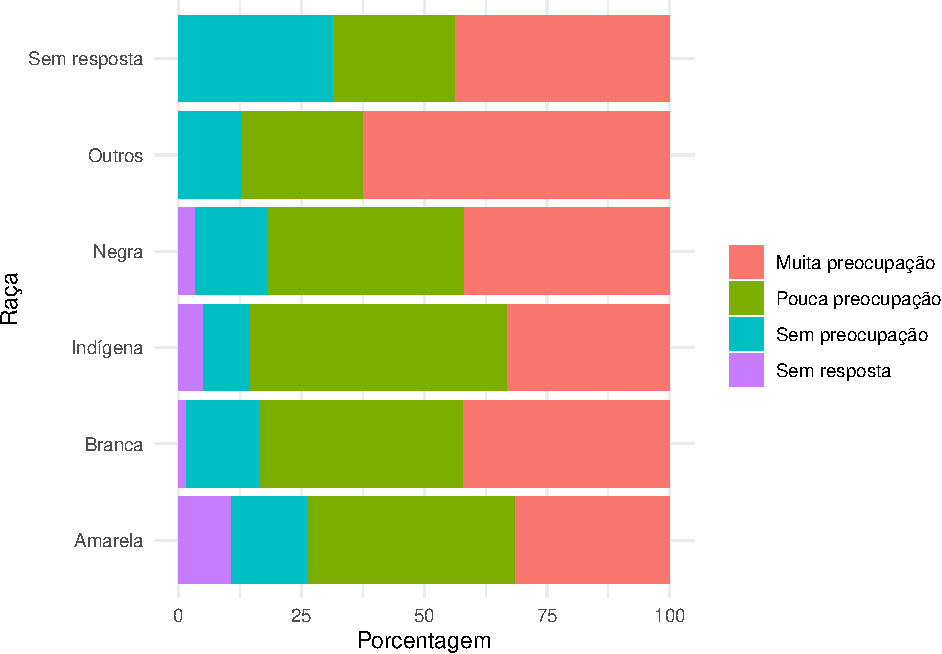
\includegraphics[width=0.75\linewidth]{relatorio_files/figure-latex/unnamed-chunk-77-1} \end{center}

\hypertarget{teste-qui-quadrado-10}{%
\paragraph{Teste qui-quadrado}\label{teste-qui-quadrado-10}}

Como o valor-p é maior que \(\alpha=0,05\), não rejeitamos \(H_0\) e não temos evidência evidência estatística que as duas variáveis estão associadas.

\begin{longtable}[]{@{}ccc@{}}
\caption{\label{tab:unnamed-chunk-78}Teste qui-quadrado entre raca e Q13.}\tabularnewline
\toprule
Estatística & Graus de liberdade & Valor-p\tabularnewline
\midrule
\endfirsthead
\toprule
Estatística & Graus de liberdade & Valor-p\tabularnewline
\midrule
\endhead
19,47 & 15 & 0,19\tabularnewline
\bottomrule
\end{longtable}

\cleardoublepage

\hypertarget{medidas-de-resumo-q13-por-rauxe7a}{%
\paragraph{Medidas de Resumo Q13 por Raça}\label{medidas-de-resumo-q13-por-rauxe7a}}

\begin{longtable}[]{@{}cccccc@{}}
\caption{\label{tab:unnamed-chunk-79}Medidas de resumo de Q13 por raca.}\tabularnewline
\toprule
Q13 & Média & Desvio Padrão & Mediana & 1 Quartil & 3 Quartil\tabularnewline
\midrule
\endfirsthead
\toprule
Q13 & Média & Desvio Padrão & Mediana & 1 Quartil & 3 Quartil\tabularnewline
\midrule
\endhead
Amarela & 1,37 & 0,90 & 1 & 1 & 2\tabularnewline
Branca & 1,30 & 0,74 & 1 & 1 & 2\tabularnewline
Indígena & 1,33 & 0,73 & 1 & 1 & 2\tabularnewline
Negra & 1,33 & 0,77 & 1 & 1 & 2\tabularnewline
Outros & 1,50 & 0,73 & 2 & 1 & 2\tabularnewline
Sem resposta & 1,12 & 0,87 & 1 & 0 & 2\tabularnewline
\bottomrule
\end{longtable}

\hypertarget{boxplot-de-q13-por-rauxe7a}{%
\paragraph{Boxplot de Q13 por Raça}\label{boxplot-de-q13-por-rauxe7a}}

\begin{center}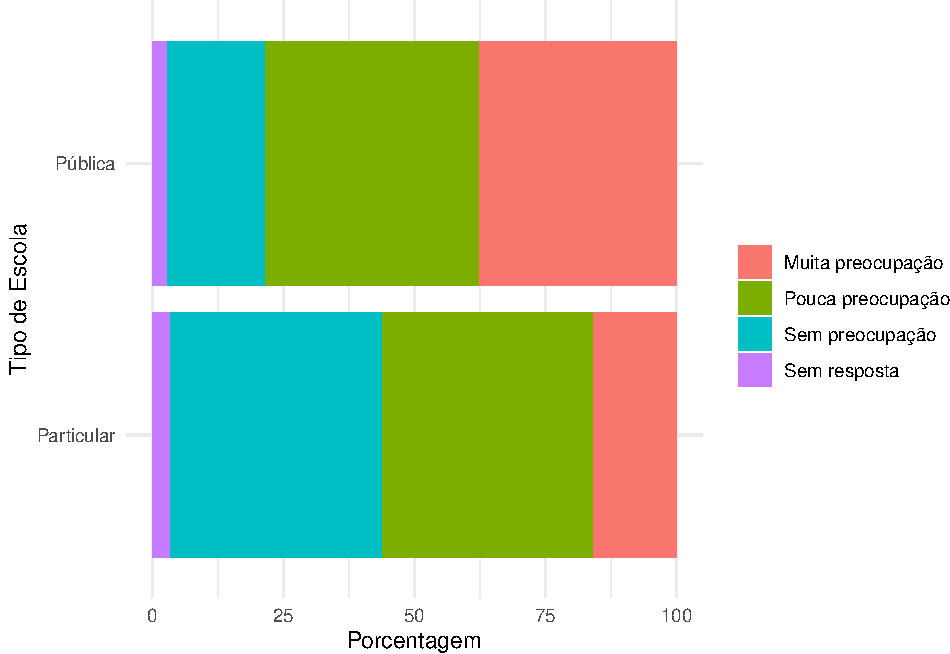
\includegraphics[width=0.75\linewidth]{relatorio_files/figure-latex/unnamed-chunk-80-1} \end{center}

\hypertarget{teste-de-kruskal-wallis-de-q13-por-rauxe7a}{%
\paragraph{Teste de Kruskal-Wallis de Q13 por Raça}\label{teste-de-kruskal-wallis-de-q13-por-rauxe7a}}

Como o valor-p é maior que \(\alpha=0,05\), não rejeitamos \(H_0\) e as medianas de \(Q13\) entre as crianças de diversas raças são iguais.

\begin{longtable}[]{@{}ccc@{}}
\caption{\label{tab:unnamed-chunk-81}Valores-p para comparação múltipla de medianas: Q13 e Raça.}\tabularnewline
\toprule
Estatística & Parâmetro & valor p\tabularnewline
\midrule
\endfirsthead
\toprule
Estatística & Parâmetro & valor p\tabularnewline
\midrule
\endhead
2,82 & 5 & 0,73\tabularnewline
\bottomrule
\end{longtable}

\hypertarget{teste-de-nemeyi-de-q13-por-rauxe7a}{%
\paragraph{Teste de Nemeyi de Q13 por Raça}\label{teste-de-nemeyi-de-q13-por-rauxe7a}}

Como o valor-p é maior que \(\alpha=0,05\), não rejeitamos \(H_0\) e as medianas de \(Q13\) entre as crianças de diversas raças são iguais.

\begin{longtable}[]{@{}lccccc@{}}
\caption{\label{tab:unnamed-chunk-82}Teste de Nemeyi de Q13 por Raça.}\tabularnewline
\toprule
& Amarela & Branca & Indígena & Negra & Outros\tabularnewline
\midrule
\endfirsthead
\toprule
& Amarela & Branca & Indígena & Negra & Outros\tabularnewline
\midrule
\endhead
Branca & 1,00 & & & &\tabularnewline
Indígena & 1,00 & 1,00 & & &\tabularnewline
Negra & 1,00 & 1,00 & 1,00 & &\tabularnewline
Outros & 0,98 & 0,89 & 0,96 & 0,93 &\tabularnewline
Sem resposta & 0,98 & 0,95 & 0,99 & 0,88 & 0,69\tabularnewline
\bottomrule
\end{longtable}

\cleardoublepage

\hypertarget{tabela-de-continguxeancia-tipo-de-escola-e-q13}{%
\paragraph{Tabela de contingência: Tipo de escola e Q13}\label{tabela-de-continguxeancia-tipo-de-escola-e-q13}}

Apenas sete crianças não estavam matriculadas na escola, e foram retiradas da análise para facilitar a análise de \emph{tipo de escola}.

\begin{longtable}[]{@{}ccccc@{}}
\caption{\label{tab:unnamed-chunk-83}Tabela de contingência: Tipo de escola e Q13.}\tabularnewline
\toprule
\begin{minipage}[b]{0.16\columnwidth}\centering
Tipo de Escola\strut
\end{minipage} & \begin{minipage}[b]{0.19\columnwidth}\centering
Muita preocupação\strut
\end{minipage} & \begin{minipage}[b]{0.19\columnwidth}\centering
Pouca preocupação\strut
\end{minipage} & \begin{minipage}[b]{0.17\columnwidth}\centering
Sem preocupação\strut
\end{minipage} & \begin{minipage}[b]{0.14\columnwidth}\centering
Sem resposta\strut
\end{minipage}\tabularnewline
\midrule
\endfirsthead
\toprule
\begin{minipage}[b]{0.16\columnwidth}\centering
Tipo de Escola\strut
\end{minipage} & \begin{minipage}[b]{0.19\columnwidth}\centering
Muita preocupação\strut
\end{minipage} & \begin{minipage}[b]{0.19\columnwidth}\centering
Pouca preocupação\strut
\end{minipage} & \begin{minipage}[b]{0.17\columnwidth}\centering
Sem preocupação\strut
\end{minipage} & \begin{minipage}[b]{0.14\columnwidth}\centering
Sem resposta\strut
\end{minipage}\tabularnewline
\midrule
\endhead
\begin{minipage}[t]{0.16\columnwidth}\centering
Particular\strut
\end{minipage} & \begin{minipage}[t]{0.19\columnwidth}\centering
254\strut
\end{minipage} & \begin{minipage}[t]{0.19\columnwidth}\centering
237\strut
\end{minipage} & \begin{minipage}[t]{0.17\columnwidth}\centering
89\strut
\end{minipage} & \begin{minipage}[t]{0.14\columnwidth}\centering
10\strut
\end{minipage}\tabularnewline
\begin{minipage}[t]{0.16\columnwidth}\centering
Pública\strut
\end{minipage} & \begin{minipage}[t]{0.19\columnwidth}\centering
186\strut
\end{minipage} & \begin{minipage}[t]{0.19\columnwidth}\centering
179\strut
\end{minipage} & \begin{minipage}[t]{0.17\columnwidth}\centering
68\strut
\end{minipage} & \begin{minipage}[t]{0.14\columnwidth}\centering
20\strut
\end{minipage}\tabularnewline
\bottomrule
\end{longtable}

\hypertarget{gruxe1fico-de-barras-tipo-de-escola-e-q13}{%
\paragraph{Gráfico de barras: Tipo de escola e Q13}\label{gruxe1fico-de-barras-tipo-de-escola-e-q13}}

Apenas sete crianças não estavam matriculadas na escola, e foram retiradas da análise para facilitar a análise de \emph{tipo de escola}.

Aparentemente as duas variáveis \emph{Tipo de Escola} e \emph{Q13} não estão associadas.

\begin{center}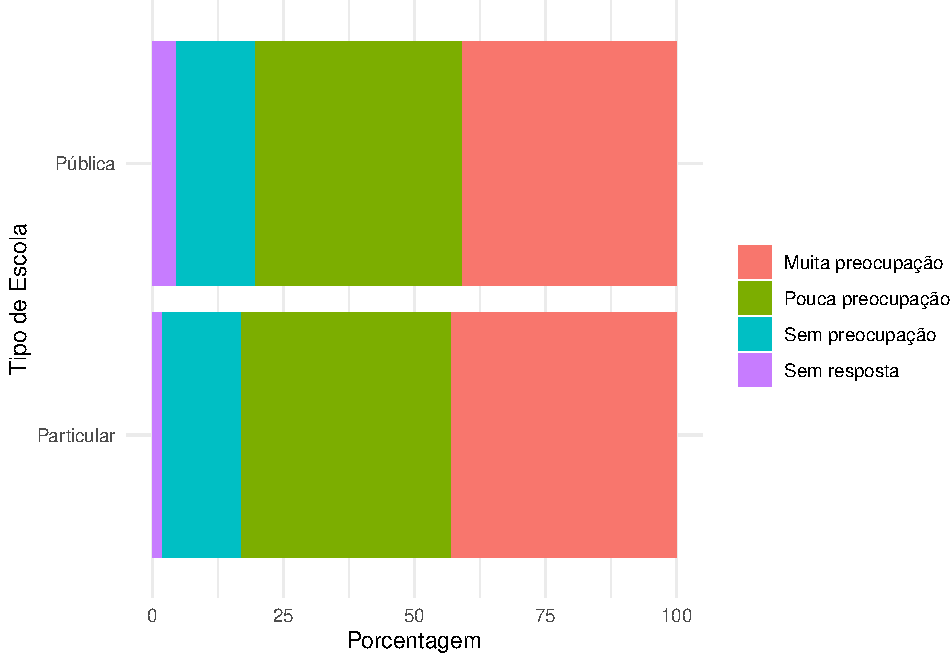
\includegraphics[width=0.75\linewidth]{relatorio_files/figure-latex/unnamed-chunk-84-1} \end{center}

\hypertarget{teste-qui-quadrado-11}{%
\paragraph{Teste qui-quadrado}\label{teste-qui-quadrado-11}}

Apenas sete crianças não estavam matriculadas na escola, e foram retiradas da análise para facilitar a análise de \emph{tipo de escola}.

Como o valor-p é menor que \(\alpha=0,05\), não rejeitamos \(H_0\) e não temos evidência evidência estatística que as duas variáveis estão associadas.

\begin{longtable}[]{@{}ccc@{}}
\caption{\label{tab:unnamed-chunk-85}Teste qui-quadrado entre Escola e Q13.}\tabularnewline
\toprule
Estatística & Graus de liberdade & Valor-p\tabularnewline
\midrule
\endfirsthead
\toprule
Estatística & Graus de liberdade & Valor-p\tabularnewline
\midrule
\endhead
6,86 & 3 & 0,08\tabularnewline
\bottomrule
\end{longtable}

\cleardoublepage

\hypertarget{medidas-de-resumo-q13-por-tipo-de-escola}{%
\paragraph{Medidas de Resumo Q13 por Tipo de escola}\label{medidas-de-resumo-q13-por-tipo-de-escola}}

Apenas sete crianças não estavam matriculadas na escola, e foram retiradas da análise para facilitar a análise de \emph{tipo de escola}.

\begin{longtable}[]{@{}cccccc@{}}
\caption{\label{tab:unnamed-chunk-86}Medidas de resumo de Q13 por Escola.}\tabularnewline
\toprule
Q13 & Média & Desvio Padrão & Mediana & 1 Quartil & 3 Quartil\tabularnewline
\midrule
\endfirsthead
\toprule
Q13 & Média & Desvio Padrão & Mediana & 1 Quartil & 3 Quartil\tabularnewline
\midrule
\endhead
Particular & 1,31 & 0,74 & 1 & 1 & 2\tabularnewline
Pública & 1,35 & 0,79 & 1 & 1 & 2\tabularnewline
\bottomrule
\end{longtable}

\hypertarget{boxplot-de-q13-por-tipo-de-escola}{%
\paragraph{Boxplot de Q13 por Tipo de escola}\label{boxplot-de-q13-por-tipo-de-escola}}

Apenas sete crianças não estavam matriculadas na escola, e foram retiradas da análise para facilitar a análise de \emph{tipo de escola}.

\begin{center}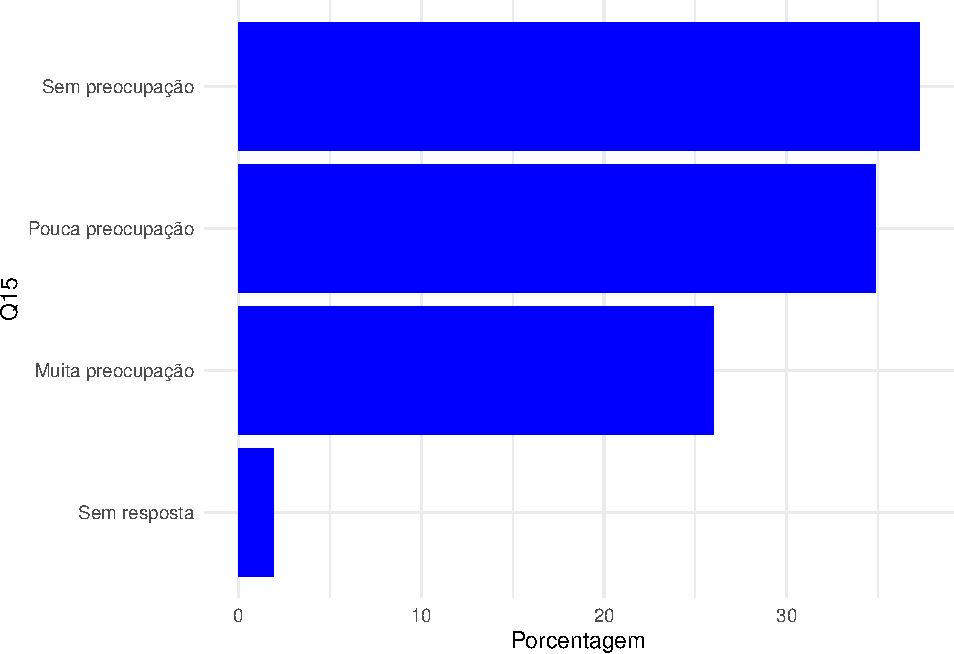
\includegraphics[width=0.75\linewidth]{relatorio_files/figure-latex/unnamed-chunk-87-1} \end{center}

\hypertarget{teste-de-kruskal-wallis-de-q13-por-tipo-de-escola}{%
\paragraph{Teste de Kruskal-Wallis de Q13 por Tipo de escola}\label{teste-de-kruskal-wallis-de-q13-por-tipo-de-escola}}

Apenas sete crianças não estavam matriculadas na escola, e foram retiradas da análise para facilitar a análise de \emph{tipo de escola}.

Como o valor-p é maior que \(\alpha=0,05\), não rejeitamos \(H_0\) e as medianas de \(Q13\) entre as escolas particulares e públicas são iguais.

\begin{longtable}[]{@{}ccc@{}}
\caption{\label{tab:unnamed-chunk-88}Valores-p para comparação múltipla de medianas: Q13 e Tipo de escola.}\tabularnewline
\toprule
Estatística & Parâmetro & valor p\tabularnewline
\midrule
\endfirsthead
\toprule
Estatística & Parâmetro & valor p\tabularnewline
\midrule
\endhead
1,14 & 1 & 0,28\tabularnewline
\bottomrule
\end{longtable}

\hypertarget{teste-de-nemeyi-de-q13-por-tipo-de-escola}{%
\paragraph{Teste de Nemeyi de Q13 por Tipo de escola}\label{teste-de-nemeyi-de-q13-por-tipo-de-escola}}

Apenas sete crianças não estavam matriculadas na escola, e foram retiradas da análise para facilitar a análise de \emph{tipo de escola}.

Como o valor-p é maior que \(\alpha=0,05\), não rejeitamos \(H_0\) e as medianas de \(Q13\) entre as escolas particulares e públicas são iguais.

\begin{longtable}[]{@{}lc@{}}
\caption{\label{tab:unnamed-chunk-89}Teste de Nemeyi de Q13 por Escola.}\tabularnewline
\toprule
& Particular\tabularnewline
\midrule
\endfirsthead
\toprule
& Particular\tabularnewline
\midrule
\endhead
Pública & 0,61\tabularnewline
\bottomrule
\end{longtable}

\cleardoublepage

\hypertarget{referuxeancias}{%
\section*{Referências}\label{referuxeancias}}
\addcontentsline{toc}{section}{Referências}

\hypertarget{refs}{}
\leavevmode\hypertarget{ref-barbetta2008estatistica}{}%
Barbetta, Pedro Alberto. 2008. \emph{Estatística Aplicada às Ciências Sociais}. Editora UFSC.

\leavevmode\hypertarget{ref-bussab2002estatistica}{}%
Bussab, Wilton de Oliveira, and Pedro Alberto Morettin. 2002. \emph{Estatística Básica. 5a Edição}. Editora Saraiva.

\leavevmode\hypertarget{ref-hollander2013nonparametric}{}%
Hollander, Myles, Douglas A Wolfe, and Eric Chicken. 2013. \emph{Nonparametric Statistical Methods}. Vol. 751. John Wiley \& Sons.

\leavevmode\hypertarget{ref-montgomery2010applied}{}%
Montgomery, Douglas C, and George C Runger. 2010. \emph{Applied Statistics and Probability for Engineers}. John Wiley \& Sons.

\leavevmode\hypertarget{ref-nemenyi1963distribution}{}%
Nemenyi, Peter Bjorn. 1963. \emph{Distribution-Free Multiple Comparisons.} Princeton University.

\leavevmode\hypertarget{ref-PMCMR}{}%
Pohlert, Thorsten. 2014. \emph{The Pairwise Multiple Comparison of Mean Ranks Package (Pmcmr)}. \url{https://CRAN.R-project.org/package=PMCMR}.

\leavevmode\hypertarget{ref-Rlang}{}%
R Core Team. 2021. \emph{R: A Language and Environment for Statistical Computing}. Vienna, Austria: R Foundation for Statistical Computing. \url{https://www.R-project.org/}.

\leavevmode\hypertarget{ref-spiegel2001probability}{}%
Spiegel, Murray R, John J Schiller, R Alu Srinivasan, and Mike LeVan. 2001. \emph{Probability and Statistics}. Vol. 2. Mcgraw-hill.

\end{document}
